\documentclass[a4paper,12pt,oneside,onecolumn,final,fleqn]{repUERJ}

\usepackage[english,brazil]{babel}  % adequação para o português Brasil
\usepackage[utf8]{inputenc} % Determina a codificação utilizada
                            % (conversão automática dos acentos)
\usepackage{makeidx}        % Cria o índice
\usepackage{hyperref}       % Controla a formação do índice
\usepackage{indentfirst}    % Endenta o primeiro paragrafo de
                            % cada seção.
\usepackage{graphicx}       % Inclusão de gráficos
\usepackage{subfig}
\usepackage{amsmath}        % pacote matemático
\usepackage{bm}             % pacote de fontes matematicas
\usepackage{lscape}         % pacote para colocar páginas em landscape
\usepackage{array}

\usepackage{float}
\usepackage{geometry}
\usepackage{pgfgantt}
\usepackage{setspace}

% ---
% Pacote auxiliar para as normas da UERJ
% ---
\usepackage[frame=no,font=default]{repUERJformat}
\usepackage[line=yes]{repUERJpseudocode} 
% ---
% Pacotes de citacoes
% ---
\usepackage[alf,abnt-repeated-author-omit=no]{abntex2cite}
% ---
\selectlanguage{brazil} 


% ********************************************************************
% ********************************************************************
% Área Reservada para incluir os novos comandos
% ********************************************************************
% ********************************************************************

% Comandos de comentários
\definecolor{green}{rgb}{0.1, 0.4, 0.1}
\newcommand\red[1]{{\color{red}#1}}
\newcommand\sred[1]{{\color{red}\uline{#1}}}
\newcommand\blue[1]{{\color{blue}#1}}
\newcommand\sblue[1]{{\color{blue}\uline{#1}}}
\newcommand\green[1]{{\color{green}#1}}
\newcommand\sgreen[1]{{\color{green}\uline{#1}}}
\newcommand\orange[1]{{\color{orange}#1}}
\newcommand\sorange[1]{{\color{orange}\uline{#1}}}
%o comando \sout funciona para riscar o texto

% ********************************************************************
% ********************************************************************
% Informações de autoria e institucionais
% ********************************************************************
% ********************************************************************

%---------------------------------------------------------------------
% Imagens pretextuais (precisam estar no mesmo diretório deste arquivo .tex)
%---------------------------------------------------------------------
 
\logo{logo_uerj_cinza.png}
\marcadagua{marcadagua_uerj_cinza.png}{1}{160}{255}

%---------------------------------------------------------------------
% Informações da instituição
%---------------------------------------------------------------------
\instituicao{Universidade do Estado do Rio de Janeiro}  %Universidade
            {Centro de Tecnologia e Ciências}  %Centro
            {Faculdade de Engenharia} %Unidade
            {} %Departamento (DEIXAR EM BRANCO)

%---------------------------------------------------------------------
% Informações da autoria do documento
%---------------------------------------------------------------------

\autor{Petro}
      {Liporace Cardoso de Souza}
      {P. L. C. de S.} % iniciais do nome

\titulo{Escalabilidade em Aplicações Globais em Tempo Real: Um Estudo de Caso com o Projeto Codeboard UERJ} %Título do trabalho acadêmico em português
\title{Scalability in Global Real-Time Applications: A Case Study with the Codeboard UERJ Project} %Título do trabalho acadêmico em inglês



\orientador{Prof.ª} %cargo, ex.: Prof., Profa., Eng. , etc...
		   {Rafaela}{Correia Brum} %Nome sobrenome com a titulação ao final. Exemplo: D.Sc., Ph.D., M.Sc., B.Sc., etc.
           {Universidade Federal Fluminense - UFF} % Instituição e Departamento ou PPG


%Opcional, Comente as linhas de coorientador caso não tenha
\coorientador{Prof.ª}  %cargo, ex.: Prof., Profa., Eng. , etc...
           {Cristiana}{Barbosa Bentes}  %Nome sobrenome com a titulação ao final. Exemplo: D.Sc., Ph.D., M.Sc., B.Sc., etc.
           {Departamento de Engenharia de Sistemas e Computação - UERJ} % Instituição e Departamento ou PPG

%---------------------------------------------------------------------
% Grau pretendido (Doutor, Mestre, Bacharel, Licenciado) e Curso
%---------------------------------------------------------------------

\newcommand\artigo{a} 

\grau{Graduação}

\curso{Engenharia Elétrica} 
\newcommand\grauTitulo{Graduado em Engenharia Elétrica}  

\areadeconcentracao{Sistemas e Computação} 

%---------------------------------------------------------------------
% Informações adicionais (local, data e paginas)
%---------------------------------------------------------------------

\local{Rio de Janeiro} 
\data{DD}{Dezembro}{2024} % Exemplo: \data{21}{Março}{2016}

% ********************************************************************
% ********************************************************************
% Configurações de aparência do PDF final
% ********************************************************************
% ********************************************************************

% alterando o aspecto da cor azul
\definecolor{blue}{RGB}{41,5,195}
%\definecolor{apricot}{RGB}{251,206,177}

% informações do PDF
\hypersetup{
  unicode=false,
  pdftitle={\UERJtitulo},
  pdfauthor={\UERJautor},
  pdfsubject={\UERJpreambulo},
  pdfkeywords={PALAVRAS}{CHAVES}{\chaveA}{\chaveB}{\chaveC}{\chaveD},
  pdfproducer={\packagename}, % producer of the document
  pdfcreator={\UERJautor},
  colorlinks=true,            % false: boxed links; true: colored links
  linkcolor=black,            % color of internal links blue
  citecolor=black,            % color of links to bibliography blue
  filecolor=black,            % color of file links magenta
  urlcolor=black,
  bookmarksdepth=4,
  %backref=true,
  %pagebackref=true,
  %bookmarks=true,
}

% ********************************************************************
% ********************************************************************
% Início do documento
% ********************************************************************
% ********************************************************************
% ---
% compila o índice; se não for usar, comentar
% ---
\makeindex
% ********************************************************************
% ********************************************************************

\selectlanguage{brazil} % setando o idioma global para português

\begin{document}
% ----------------------------------------------------------
%% ELEMENTOS PRE-TEXTUAIS
% ----------------------------------------------------------
\frontmatter

\capa
\folhaderosto

% ----------------------------------------------------------
% Inserir a ficha catalográfica
% ----------------------------------------------------------
% ---
% A biblioteca deverá providenciar a ficha catalográfica. Salve a ficha no
% formato PDF. Use o nome do arquivo PDF como argumento do comando. 
% Exemplo: ficha catalográfica é o arquivo 'Ficha.pdf' na pasta "pre-textual"
%     \fichacatalografica{pre-textual/Ficha.pdf}
%
% Enquanto não possuir a ficha catalográfica, use o comando sem argumentos.
% ---
\fichacatalografica{pre-textual/Ficha.pdf}

% ----------------------------------------------------------
% Folha de aprovação

%Após obter a assinatura dos membros da banca, comente as linhas a baixos e insira o pdf com as assinaturas na pasta "pre-textual"


% Ajustar o espaço entre as assinaturas abaixo
\newcommand{\spc}{0.25cm}

\begin{folhadeaprovacao}
	\vspace{\spc} % Espaço entre assinaturas
	\assinatura{Prof. Giomar Oliver Sequeiros Olivera}{Departamento de Engenharia de Sistemas e Computação - UERJ} %Exemplo
	\vspace{\spc} % Espaço entre assinaturas
	\assinatura{Prof. Thiago Medeiros Carvalho}{Departamento de Engenharia de Sistemas e Computação - UERJ}
\end{folhadeaprovacao}


% Após colocar o pdf com as assinaturas na pasta "pre-textual", comente todo o ambiente "folhadeaprovacao" acima, descomente a linha abaixo e insira o nome correto do arquivo pdf:
%\includepdf[pages=1]{pre-textual/ficha.pdf} %exemplo

% Dedicatória
\pretextualchapter{Dedicatória}
\vfill
Eu dedico essa tese para uma pessoa muito especial.






% Agradecimentos
\pretextualchapter{Agradecimentos}

Gostaria de expressar minha mais profunda gratidão a todos que, de alguma forma, contribuíram para a realização deste trabalho e para a conclusão da minha graduação.

Primeiramente, à minha mãe, Luzia Magalhães, pelo apoio incondicional ao longo de toda a minha trajetória acadêmica. Suas palavras de incentivo e seu entusiasmo com cada uma das minhas conquistas foram essenciais para que eu pudesse alcançar este momento tão significativo.

À Ketlin Rodrigues, por estar sempre ao meu lado, oferecendo suporte emocional e sendo uma presença constante de carinho e compreensão nos momentos mais desafiadores. Sua parceria foi indispensável nesta caminhada.

Aos meus amigos João Pedro Costa, Jorge dos Santos, Mayara Rodrigues, Rodrigo Tak-Ming, Gabriel Vidile e tantos outros que fizeram parte desta jornada, proporcionando momentos de alegria, suporte e colaboração inestimáveis.

Um agradecimento especial ao meu amigo Rafael Chrispim, que, mesmo não estando mais entre nós, deixou uma marca permanente em minha vida. Sua amizade, apoio e incentivo continuam a me inspirar e foram fundamentais para que eu me tornasse a pessoa que sou hoje.

À Growth Machine, empresa da qual sou sócio, pela flexibilidade e compreensão que me permitiram equilibrar meus compromissos profissionais e acadêmicos, proporcionando o espaço necessário para que eu pudesse crescer em ambos os campos.

À UERJ, ao Departamento de Sistemas e Computação e às minhas orientadoras, Rafaela e Cristiana, pela orientação e pelo suporte acadêmico ao longo deste percurso. A dedicação de vocês foi essencial para a realização deste trabalho e para o meu desenvolvimento como profissional.

A todos vocês, os meus mais sinceros agradecimentos. Cada um, de sua forma particular e única, contribuiu para que eu chegasse até aqui e para a minha trajetória profissional. Este TCC é um marco e também o reflexo de tudo o que aprendi e vivenciei ao lado de vocês.


% Epigrafe (opcional)
\pretextualchapter{}
\vfill
\begin{flushright}
	"Nada é permanente, exceto a mudança."\\
	\textit{Heráclito de Éfeso}
\end{flushright}










%% RESUMO
% se não for usar a quarta palavra chave, deixar o campo vazio: {}
\palavraschaves{Escalabilidade}
{Computação em nuvem}
{Aplicações em tempo real}
{WebSockets}


\pretextualchapter{Resumo}
\referencia % linha em branco depois

Desde a popularização da internet, a escalabilidade em aplicações globais tem se tornado um desafio crescente, especialmente com a popularização de tecnologias que fornecem interações em tempo real entre usuários. O presente trabalho explora os desafios e soluções de escalabilidade nessas aplicações, utilizando como estudo de caso a plataforma Codeboard UERJ. Desenvolvida para o ensino remoto, a Codeboard oferece um ambiente de programação colaborativa em tempo real, permitindo interações simultâneas entre professores e alunos. O estudo aborda conceitos fundamentais de desenvolvimento web, computação em nuvem e comunicação em tempo real, bem como a implementação de práticas avançadas de escalabilidade horizontal e vertical, balanceamento de carga e tolerância a falhas. A infraestrutura cloud foi projetada para lidar com altas demandas, empregando tecnologias como WebSockets, MongoDB, Redis e Auto Scaling. Os testes realizados demonstraram a eficácia das estratégias implementadas, assegurando desempenho consistente e confiabilidade mesmo sob condições adversas. Este trabalho contribui para o avanço da engenharia de sistemas distribuídos e serve como referência prática para desenvolvedores e arquitetos de software interessados em soluções escaláveis e com alta disponibilidade.


\imprimirchaves % linha em branco antes




% Abstract
\begin{otherlanguage}{english}
\keywords{first keyword}
{second keyword}
{third keyword}
{fourth keyword (if any)}


\pretextualchapter{Abstract}
\reference % linha em branco depois

% O resumo em inglês deve ser organizado em apenas um parágrafo mesmo.

 Happiness deserves a English description. Lorem ipsum dolor sit amet, consectetur adipiscing elit, sed do eiusmod tempor incididunt ut labore et dolore magna aliqua. Ut enim ad minim veniam, quis nostrud exercitation ullamco laboris nisi ut aliquip ex ea commodo consequat. Duis aute irure dolor in reprehenderit in voluptate velit esse cillum dolore eu fugiat nulla pariatur. Excepteur sint occaecat cupidatat non proident, sunt in culpa qui officia deserunt mollit anim id est laborum. Sed ut perspiciatis unde omnis iste natus error sit voluptatem accusantium doloremque laudantium, totam rem aperiam, eaque ipsa quae ab illo inventore veritatis et quasi architecto beatae vitae dicta sunt explicabo. Nemo enim ipsam voluptatem quia voluptas sit aspernatur aut odit aut fugit, sed quia consequuntur magni dolores eos qui ratione voluptatem sequi nesciunt. Neque porro quisquam est, qui dolorem ipsum quia dolor sit amet, consectetur, adipisci velit, sed quia non numquam eius modi tempora incidunt ut labore et dolore magnam aliquam quaerat voluptatem. Ut enim ad minima veniam, quis nostrum exercitationem ullam corporis suscipit laboriosam, nisi ut aliquid ex ea commodi consequatur? Quis autem vel eum iure reprehenderit qui in ea voluptate velit esse quam nihil molestiae consequatur, vel illum qui dolorem eum fugiat quo voluptas nulla pariatur?
 
 xxxxxxxxxxxxxxxxxxxxxxxxxxxx xxxxxxxxxxxxxxxxxxx Hyphenation test: monumental bla bla bla \\

\printkeys % linha em branco antes


\end{otherlanguage}


% ----------------------------------------------------------
% Listas de ilustrações, tabelas e algoritmos
% ----------------------------------------------------------
\listadefiguras
\listadetabelas
%\listadealgoritmos

% ----------------------------------------------------------
% Lista de abreviaturas, siglas e símbolos	
% \pretextualchapter{Lista de abreviaturas e siglas}
% ---
\abreviatura{CITT}{Técnica da Transformada integral Clássica}
\abreviatura{GITT}{Técnica da Transformada integral Generalizada}
\abreviatura{MVF}{Método de Volumes Finitos}








% \pretextualchapter{Lista de símbolos}
% ---
\simbolo{t}{Tempo}
\simbolo{L}{Dimensão na direção $x$}
\simbolo{H}{Dimensão na direção $y$}
\simbolo{\rho}{Massa específica}
\simbolo{\mu}{Viscosidade dinâmica}
\simbolo{\nu}{Viscosidade cinemática}








% ----------------------------------------------------------

\sumario

% ----------------------------------------------------------
%% ELEMENTOS TEXTUAIS
% ----------------------------------------------------------
\mainmatter

\chapter*{Introdução}

Na era digital em que vivemos, as aplicações em tempo real tornaram-se um componente crucial que conecta a sociedade moderna. Durante a pandemia de COVID-19, a necessidade de ferramentas digitais interativas e de qualidade tornou-se ainda mais evidente, especialmente no campo educacional\cite{impact-covid19-teaching-learning}. Com o fechamento das instituições de ensino e a transição para o formato remoto, tecnologias capazes de oferecer colaboração em tempo real ganharam destaque como elementos essenciais para manter a continuidade do aprendizado.

A escalabilidade, nesse cenário, se mostra como um dos maiores desafios técnicos para o desenvolvimento de sistemas globais, pois é necessário atender a um número crescente de usuários e à crescente complexidade das interações em tempo real. Soluções robustas em computação em nuvem e estratégias de paralelismo têm se mostrado indispensáveis para superar esses obstáculos e garantir desempenho e confiabilidade mesmo em condições de alta demanda.

Este projeto de graduação tem como objetivo explorar as nuances da escalabilidade em aplicações globais em tempo real, com foco na análise e desenvolvimento da plataforma Codeboard UERJ. Voltada para o ensino de programação, a plataforma permite a colaboração simultânea de professores e alunos por meio de um ambiente de codificação interativo e dinâmico. Ao longo do trabalho, serão investigadas práticas e estratégias que garantem uma infraestrutura capaz de se adaptar à demanda, mantendo um alto nível de desempenho e confiabilidade.

Ao documentar os desafios enfrentados e as soluções implementadas, este estudo busca contribuir para a compreensão e o avanço da engenharia de sistemas em larga escala. Além disso, espera-se que os insights obtidos sirvam como referência prática para desenvolvedores, arquitetos de sistemas e tomadores de decisão, promovendo a excelência na entrega de serviços em tempo real e fortalecendo a conexão entre tecnologia e educação.

Nos capítulos que seguem, serão apresentados os fundamentos teóricos que embasam este trabalho, incluindo conceitos de desenvolvimento web, computação em nuvem e protocolos de comunicação. Em seguida, será detalhada a arquitetura e implementação da plataforma Codeboard UERJ, abordando as estratégias adotadas para garantir sua robustez e eficiência. Os capítulos posteriores trarão uma análise dos testes realizados, os resultados obtidos e as discussões sobre as soluções implementadas. Por fim, serão destacadas as conclusões alcançadas e as perspectivas para trabalhos futuros.
\section{Conceitos Básicos}
% 🆗 Revisado

Antes de aprofundar nos aspectos técnicos específicos deste trabalho, é fundamental entender os conceitos que sustentam o desenvolvimento de aplicações web e a computação em nuvem. Este capítulo apresenta de forma sucinta esses conceitos básicos, fornecendo uma base para a compreensão das tecnologias e práticas utilizadas na construção e operação de aplicações web modernas.

\subsection{Desenvolvimento Web}
% 🆗 Revisado

O desenvolvimento web é a área da engenharia de computação que se dedica à criação de aplicações e serviços acessíveis através da internet. Envolve a construção de sites, aplicações web e outras soluções online que interagem com usuários por meio de navegadores ou dispositivos conectados.

\subsubsection{Aplicações Web}
% 🆗 Revisado

% O que são aplicações web?
% Que tecnologias são utilizadas para desenvolver aplicações web? (HTML, CSS, JavaScript, etc.)

Aplicações web são programas ou sistemas desenvolvidos para serem executados em navegadores de internet, permitindo que usuários acessem funcionalidades e informações através da web. Diferentemente dos softwares tradicionais instalados localmente, as aplicações web podem ser acessadas de qualquer lugar com conexão à internet, facilitando a distribuição e atualização.

Para desenvolver aplicações web, utilizam-se diversas tecnologias que colaboram entre si:

\begin{itemize}
    \item \textbf{HTML (HyperText Markup Language)}: Linguagem de marcação responsável por estruturar o conteúdo da web.
    \item \textbf{CSS (Cascading Style Sheets)}: Linguagem de estilo utilizada para definir a aparência e o layout dos documentos HTML.
    \item \textbf{JavaScript}: Linguagem de programação que permite adicionar interatividade e dinamismo às páginas web.
\end{itemize}

Essas tecnologias constituem a base do desenvolvimento web front-end, proporcionando interfaces amigáveis e funcionais para os usuários.

\subsubsection{Front-end e Back-end}
% 🆗 Revisado

% O que é front-end?
% O que é back-end?
% Qual a diferença entre front-end e back-end?
% Como se comunicam? (via HTTP por meio de APIs, via WebSockets, etc.)

No desenvolvimento de aplicações web, a arquitetura é geralmente dividida em duas camadas principais:

\begin{itemize}
    \item \textbf{Front-end}: Refere-se à parte da aplicação que interage diretamente com o usuário. Inclui tudo o que o usuário vê e com o que interage no navegador, como layouts, botões e formulários. Tecnologias como HTML, CSS e JavaScript, além de frameworks como React.js, são comumente utilizadas.
    \item \textbf{Back-end}: É a camada de servidor da aplicação, responsável pelo processamento de dados, lógica de negócio e comunicação com bancos de dados. Tecnologias como Node.js, Go, Java e frameworks como Express.js são utilizadas para desenvolver o back-end.
\end{itemize}

A comunicação entre o front-end e o back-end ocorre por meio de protocolos como HTTP. O front-end envia requisições ao back-end, que processa os dados e retorna respostas, geralmente via APIs. Em aplicações em tempo real, tecnologias como WebSockets também são utilizadas para comunicação bidirecional persistente entre cliente e servidor.

\subsubsection{APIs}
% 🆗 Revisado

% O que é uma API?
% Quais são os tipos de APIs? (REST, GraphQL, etc.)
% O que é REST?

Uma \emph{API (Application Programming Interface)}  é um conjunto de definições e protocolos que permite a comunicação entre diferentes softwares. No contexto de aplicações web, as APIs desempenham um papel crucial ao possibilitar a interação entre o front-end e o back-end, permitindo operações como a obtenção de dados e a execução de ações no servidor.

Existem vários tipos de APIs, sendo atualmente dois dos mais populares:

\begin{itemize}
    \item \textbf{REST (Representational State Transfer)}:Um estilo arquitetural baseado no protocolo HTTP que oferece uma interface uniforme para manipulação de recursos. É amplamente adotado por sua simplicidade e aderência aos padrões da web, facilitando a integração entre sistemas.
    \item \textbf{GraphQL}: Uma linguagem de consulta para APIs que permite solicitar exatamente os dados necessários, melhorando a eficiência e reduzindo a quantidade de informações transferidas nas requisições.
\end{itemize}

Ambos os padrões são amplamente utilizados, com o \emph{REST} sendo preferido em muitos casos devido à sua simplicidade, enquanto o GraphQL se destaca em cenários que demandam maior flexibilidade na recuperação de dados.


\subsubsection{Node.js}
% 🆗 Revisado

% O que é Node.js?
% Quais são as vantagens de utilizar Node.js para desenvolver aplicações web?

\emph{Node.js} é um ambiente de execução de JavaScript projetado para o desenvolvimento do lado do servidor (back-end). Ele permite que os desenvolvedores utilizem JavaScript fora do navegador, possibilitando a criação de aplicações escaláveis, de alto desempenho e adequadas para diferentes tipos de cenários, como APIs, sistemas em tempo real e microsserviços.

Construído sobre o motor V8 do Google Chrome, o Node.js oferece execução extremamente rápida para código JavaScript. Ele adota um modelo de programação assíncrono e orientado a eventos, ideal para lidar com operações intensivas de entrada e saída, como comunicação com bancos de dados ou requisições HTTP.

Vantagens de utilizar Node.js para desenvolver aplicações web:

\begin{itemize}
    \item \textbf{Modelo assíncrono e orientado a eventos}: O modelo non-blocking permite que o servidor lide com múltiplas conexões simultaneamente, tornando-o altamente eficiente e ideal para aplicações que demandam grande escalabilidade, como chats em tempo real e streaming de dados.
    \item \textbf{Comunidade ativa e ecossistema rico}: A comunidade do Node.js é uma das mais movimentadas no desenvolvimento de software, e o NPM (Node Package Manager) disponibiliza milhões de módulos e bibliotecas prontos para uso, agilizando o desenvolvimento e aumentando a produtividade.
    \item \textbf{Unificação da linguagem}: O uso do JavaScript tanto no front-end quanto no back-end elimina a necessidade de lidas com linguagens diferentes para cada camada da aplicação, promovendo maior consistência e redução de complexidade.
\end{itemize}

Além disso, o Node.js é frequentemente escolhido para projetos modernos devido à sua flexibilidade e capacidade de suportar arquiteturas orientadas a microsserviços, permitindo que equipes desenvolvam e mantenham aplicações robustas com maior eficiência.

\subsubsection{Bibliotecas e Frameworks}
% 🆗 Revisado

% O que são frameworks? E bibliotecas? Qual a diferença entre eles?
% O que é React.js?
% O que é Next.js?
% O que é Express.js?

Frameworks e bibliotecas são ferramentas essenciais no desenvolvimento de software, amplamente empregadas para acelerar a criação de aplicações.

Bibliotecas consistem em coleções de funções ou componentes reutilizáveis que os desenvolvedores incorporam em seus projetos para resolver problemas específicos. Ao contrário dos frameworks, as bibliotecas não impõem uma estrutura fixa ao projeto, proporcionando maior flexibilidade e controle ao desenvolvedor sobre como e quando utilizá-las. Um exemplo notável é o React.js, uma biblioteca focada na criação de interfaces de usuário. Ela permite o uso de componentes reutilizáveis e oferece mecanismos eficientes para o gerenciamento de estados.

Frameworks, por sua vez, fornecem uma estrutura completa para o desenvolvimento de aplicações. Eles estabelecem uma arquitetura definida e um fluxo de trabalho consistente, além de integrarem um conjunto robusto de ferramentas para tarefas como roteamento, renderização e manipulação de requisições. Entre os frameworks mais populares, destacam-se:
\begin{itemize}
    \item \textbf{Next.js}: Um framework baseado em React que introduz funcionalidades avançadas, como renderização no lado do servidor (SSR) e geração de sites estáticos (SSG), otimizando o desempenho e melhorando a SEO.
    \item \textbf{Express.js}: Um framework minimalista para Node.js, projetado para simplificar o desenvolvimento de aplicações web e APIs. Ele facilita o gerenciamento de rotas, requisições e middlewares.
\end{itemize}

Tanto bibliotecas quanto frameworks desempenham um papel crucial no desenvolvimento de software. Essas ferramentas não apenas aceleram o processo de criação, mas também incentivam a adoção de boas práticas, contribuindo para a eficiência e qualidade dos projetos.


\subsection{Protocolos de Comunicação}
% 🆗 Revisado

Protocolos de comunicação são conjuntos de regras e convenções que determinam como os dados são transmitidos e recebidos entre sistemas. Esses protocolos desempenham um papel fundamental na garantia da interoperabilidade e integração entre os diversos componentes de um sistema distribuído, permitindo que diferentes tecnologias e dispositivos trabalhem juntos de maneira eficiente e coordenada.

\subsubsection{HTTP}
% 🆗 Revisado

O \emph{HTTP (Hypertext Transfer Protocol)} é o protocolo base da web, utilizado para a comunicação entre clientes (como navegadores) e servidores. Ele define as regras para formatação e transmissão de mensagens, bem como as ações que devem ser executadas em resposta a diferentes comandos.

O HTTP segue o modelo de requisição-resposta, no qual o cliente envia uma requisição ao servidor, que, por sua vez, processa a solicitação e retorna uma resposta. Tanto as requisições quanto as respostas são compostas por cabeçalhos, que contêm informações importantes, e, opcionalmente, por um corpo que transporta dados adicionais.

Entre os métodos HTTP mais utilizados, destacam-se:

\begin{itemize}
    \item \textbf{GET}: Utilizado para solicitar a representação de um recurso sem modificar seus dados.
    \item \textbf{POST}: Envia dados ao servidor para serem processados, frequentemente utilizado em formulários e envio de informações.
    \item \textbf{PUT}: Atualiza ou substitui a representação de um recurso existente.
    \item \textbf{DELETE}: Remove um recurso especificado.
\end{itemize}

O HTTP é fundamental para o funcionamento da web, permitindo a interação entre clientes e servidores de forma padronizada e eficiente.

\subsubsection{WebSockets}
% 🆗 Revisado

\emph{WebSocket} é um protocolo de comunicação que permite uma interação bidirecional e em tempo real entre cliente e servidor por meio de uma única conexão TCP. Ele foi projetado para superar as limitações do protocolo HTTP, que é baseado no modelo de requisição-resposta e não mantém uma conexão persistente.

Ao contrário do HTTP, onde o cliente precisa iniciar cada requisição para receber novos dados, os WebSockets mantêm a conexão ativa após o handshake inicial. Isso possibilita que tanto o cliente quanto o servidor enviem mensagens de forma independente e assíncrona, sem a necessidade de estabelecer novas conexões para cada troca de dados. 

Características principais do WebSocket:

\begin{itemize}
    \item \textbf{Comunicação em tempo real}: Permite atualizações instantâneas de dados entre cliente e servidor, ideal para aplicações que demandam respostas rápidas, como chats, jogos online e sistemas de monitoramento.
    \item \textbf{Baixa latência}: Por evitar a sobrecarga de abertura e fechamento de conexões repetidas, o WebSocket reduz significativamente a latência, tornando-o mais eficiente que alternativas baseadas em HTTP.
    \item \textbf{Conexão persistente}: Uma única conexão é mantida ativa durante toda a interação, reduzindo o consumo de recursos do servidor e melhorando a escalabilidade.
    \item \textbf{Flexibilidade no transporte de dados}: Oferece suporte tanto para mensagens em texto quanto em formato binário, atendendo a uma ampla variedade de casos de uso.
\end{itemize}

Os WebSockets transformaram a forma como aplicações modernas lidam com comunicação em tempo real, oferecendo uma solução eficiente e flexível para cenários que demandam alta interatividade e respostas imediatas. Sua capacidade de manter conexões persistentes com baixa latência torna o protocolo indispensável em sistemas que exigem troca contínua de dados, consolidando-o como uma escolha estratégica para o desenvolvimento de aplicações robustas e escaláveis.

\subsection{Banco de Dados}
% TODO: Escrever Intro


\subsubsection{SQL}
% 🆗 Revisado

\emph{SQL (Structured Query Language)} é a linguagem padrão para gerenciamento de bancos de dados relacionais. Bancos de dados SQL organizam os dados em tabelas estruturadas com esquemas predefinidos, permitindo consultas complexas, manipulação eficiente de dados e garantindo consistência por meio de transações.

Os bancos de dados baseados em SQL são amplamente utilizados devido à sua capacidade de lidar com grandes volumes de informações e à aderência a padrões que favorecem a interoperabilidade entre diferentes sistemas.

Exemplos de bancos de dados SQL:

\begin{itemize}
    \item \textbf{MySQL}: Um sistema de gerenciamento de banco de dados relacional de código aberto amplamente utilizado, especialmente em aplicações web. Ele é conhecido por sua simplicidade, desempenho e grande comunidade de suporte.
    \item \textbf{PostgreSQL}: Reconhecido por sua robustez e recursos avançados, como suporte a tipos de dados personalizados, índices complexos e transações ACID. É ideal para aplicações críticas que demandam alta confiabilidade.
    \item \textbf{SQLite}: Um banco de dados leve e embutido, que não requer um servidor dedicado. Ele é bastante utilizado em dispositivos móveis e aplicativos locais devido à sua portabilidade e simplicidade.
\end{itemize}

Os bancos de dados SQL continuam sendo a espinha dorsal de muitos sistemas corporativos e de produção, graças à sua eficiência, consistência e maturidade no mercado.

\subsubsection{NoSQL}
% 🆗 Revisado

% O que é NoSQL?
% Quais são os tipos de bancos de dados NoSQL? (Documentos, Chave-Valor, Colunas, Grafos)

\emph{NoSQL} é um termo que engloba uma categoria de sistemas de gerenciamento de banco de dados que não seguem o modelo relacional tradicional. Esses bancos de dados são projetados para lidar com grandes volumes de dados distribuídos, altamente escaláveis e frequentemente não estruturados. Eles oferecem maior flexibilidade para modelagem de dados e são amplamente utilizados em aplicações modernas, como redes sociais, IoT e análise de big data.

Principais tipos de bancos de dados NoSQL:

\begin{itemize}
    \item \textbf{Documentos}: Armazenam dados em formato de documentos, frequentemente similares ao JSON, permitindo flexibilidade na estrutura dos dados. Exemplos: MongoDB, Couchbase.
    \item \textbf{Chave-Valor}: Funcionam como um dicionário simples, onde cada chave está associada a um valor. São ideais para casos de uso como caches e armazenamento de sessões. Exemplos: Redis, DynamoDB.
    \item \textbf{Colunas}: Organizam os dados em colunas em vez de linhas, otimizando operações de leitura e escrita em larga escala. São frequentemente utilizados em sistemas de análise. Exemplos: Cassandra, HBase.
    \item \textbf{Grafos}: Focados nas relações entre os dados, utilizam nós para representar entidades e arestas para as conexões entre elas. São ideais para aplicações como redes sociais, mecanismos de recomendação e análise de conexões. Exemplos: Neo4j, ArangoDB.
\end{itemize}

Os bancos de dados NoSQL se destacam por sua capacidade de lidar com dados dinâmicos e escalar horizontalmente, oferecendo soluções sob medida para desafios específicos que muitas vezes não podem ser abordados de forma eficiente por bancos de dados relacionais tradicionais.

\subsubsection{MongoDB}
% 🆗 Revisado

\emph{MongoDB} é um banco de dados NoSQL orientado a documentos que armazena os dados no formato BSON (uma extensão binária do JSON). Ele proporciona grande flexibilidade na modelagem de dados, sendo especialmente adequado para aplicações que demandam alta escalabilidade, desempenho e a capacidade de lidar com estruturas de dados dinâmicas ou não estruturadas.

\subsubsection{Redis}
% 🆗 Revisado

\emph{Redis} é um banco de dados em memória do tipo chave-valor, amplamente utilizado como banco de dados, cache e broker de mensagens. Ele oferece suporte a estruturas de dados avançadas, como strings, hashes, listas e conjuntos ordenados, garantindo alta performance e baixa latência, características que o tornam ideal para aplicações que exigem respostas rápidas e processamento eficiente.


\subsubsection{ORMs e ODMs}
% 🆗 Revisado

\emph{ORM (Object-Relational Mapping)} e \emph{ODM (Object-Document Mapping)} são técnicas que permitem mapear objetos do código-fonte para estruturas de bancos de dados relacionais e NoSQL, respectivamente. Elas têm como objetivo simplificar a interação com os bancos de dados, permitindo que os desenvolvedores trabalhem diretamente com a linguagem de programação utilizada no projeto, em vez de escrever consultas SQL ou comandos específicos para cada tipo de banco.

\begin{itemize}
    \item \textbf{ORMs}: Facilitam a manipulação de dados em bancos de dados relacionais, abstraindo consultas SQL e permitindo o uso de objetos. Exemplo: Sequelize.
    \item \textbf{ODMs}: Executam uma função semelhante para bancos de dados NoSQL orientados a documentos, integrando objetos de forma transparente. Exemplo: Mongoose.
\end{itemize}

Essas ferramentas aumentam a produtividade ao abstrair a complexidade das operações de banco de dados, proporcionando uma camada intermediária que simplifica a manipulação de dados e facilita a integração entre a aplicação e o banco.

\subsection{Computação em Nuvem}
% 🆗 Revisado

% O que é computação em nuvem?
% Quais são os tipos de serviços de computação em nuvem? (IaaS, PaaS, SaaS)
% Quais são os principais provedores de serviços de computação em nuvem? (AWS, Google Cloud, Azure, etc.)

A computação em nuvem refere-se à entrega de serviços de computação por meio da internet, permitindo o acesso a recursos de maneira flexível, escalável e sob demanda. Essa abordagem elimina a necessidade de investir em infraestrutura física, oferecendo maior agilidade e eficiência operacional para empresas e indivíduos.

Tipos de serviços de computação em nuvem:

\begin{itemize}
    \item \textbf{IaaS (Infrastructure as a Service)}: Proporciona acesso a infraestrutura básica, como servidores, armazenamento e redes. Os usuários têm controle total sobre o ambiente, configurando e gerenciando conforme suas necessidades. Exemplos: Amazon EC2, Google Compute Engine.
    \item \textbf{PaaS (Platform as a Service)}: Oferece plataformas completas para desenvolvimento e implantação de aplicações, abstraindo a complexidade da infraestrutura subjacente. Ideal para acelerar o desenvolvimento e focar na aplicação. Exemplos: Vercel, Heroku.
    \item \textbf{SaaS (Software as a Service)}: Disponibiliza aplicativos prontos para uso por meio da internet, eliminando a necessidade de instalação ou manutenção local. É amplamente utilizado para produtividade, colaboração e gerenciamento de negócios. Exemplos: Google Drive, Salesforce.
\end{itemize}

Entre os principais provedores de serviços de computação em nuvem, destacam-se a \emph{Amazon Web Services (AWS)}, a \emph{Google Cloud Platform} e a \emph{Microsoft Azure}. Essas plataformas oferecem uma ampla gama de serviços e soluções que atendem às necessidades de empresas de diferentes tamanhos, desde \emph{startups} até grandes corporações.

\subsubsection{Amazon Web Services (AWS)}
% 🆗 Revisado

% O que é AWS?
% Quais são os principais serviços da AWS? (EC2, S3, RDS, etc.)

A \emph{Amazon Web Services (AWS)} é uma plataforma líder em computação em nuvem, oferecida pela Amazon. Ela fornece uma ampla gama de serviços, incluindo infraestrutura, poder computacional, armazenamento, banco de dados e distribuição de conteúdo, operando em escala global. A AWS é amplamente utilizada por empresas de diferentes tamanhos devido à sua flexibilidade, escalabilidade e confiabilidade.

Dentre os serviços mais populares da AWS, destacam-se:

\begin{itemize}
    \item \textbf{EC2 (Elastic Compute Cloud)}: Serviço de computação que permite criar instâncias de servidores virtuais na nuvem, oferecendo flexibilidade para dimensionar o poder computacional conforme necessário.
    \item \textbf{S3 (Simple Storage Service)}: Um serviço de armazenamento de objetos que combina alta escalabilidade, segurança e custo acessível, adequado para armazenamento de arquivos, backups e grandes volumes de dados.
    \item \textbf{RDS (Relational Database Service)}: Serviço gerenciado que simplifica a configuração, operação e escalabilidade de bancos de dados relacionais, suportando motores populares como MySQL, PostgreSQL, e SQL Server.
\end{itemize}

A AWS se destaca como uma solução estratégica para organizações que buscam inovação, escalabilidade e alta disponibilidade em suas operações na nuvem. Com uma vasta gama de serviços gerenciados e um ecossistema robusto, a plataforma permite que empresas de todos os portes implementem soluções personalizadas de forma eficiente e segura.

\subsubsection{Instâncias EC2}
% 🆗 Revisado

% O que é uma instância EC2?
% O que são tipos de instâncias EC2? (T2, M5, C5, etc.)

Uma instância EC2 (\emph{Elastic Compute Cloud}) é uma máquina virtual fornecida pela AWS que oferece capacidade computacional na nuvem. Essas instâncias permitem que usuários executem aplicações com flexibilidade e escalabilidade, sem a necessidade de gerenciar hardware físico. A AWS oferece uma ampla variedade de tipos de instâncias para atender às diferentes demandas de desempenho, custo e funcionalidade.

Os tipos de instâncias EC2 mais comuns incluem:

\begin{itemize}
    \item \textbf{T2/T3}: Instâncias de uso geral com capacidade de \emph{burst}, projetadas para cargas de trabalho com variação no uso de CPU, como pequenos servidores web e ambientes de desenvolvimento.
    \item \textbf{M5}: Instâncias de uso geral balanceadas, ideais para uma ampla gama de aplicações, como bancos de dados pequenos e servidores de médio porte.
    \item \textbf{C5}: Instâncias otimizadas para computação, desenvolvidas para tarefas que exigem alto desempenho de CPU, como simulações científicas e processamento intensivo de dados.
\end{itemize}

Cada tipo de instância oferece opções configuráveis em termos de número de vCPUs, memória e armazenamento, permitindo que os usuários escolham a melhor solução para suas necessidades específicas de computação.

\subsubsection{Escalabilidade}
% 🆗 Revisado

% O que é escalabilidade vertical?
% Como funciona a escalabilidade vertical? Quais são seus desafios?
% Quais são as vantagens da escalabilidade vertical?

% O que é escalabilidade horizontal?
% Como funciona a escalabilidade horizontal? Quais são seus desafios?
% Quais são as vantagens da escalabilidade horizontal?

Escalabilidade é a capacidade de um sistema de adaptar-se ao aumento da carga de trabalho, mantendo seu desempenho através da adição de recursos. Existem dois principais tipos de escalabilidade: vertical e horizontal.

A escalabilidade vertical consiste em melhorar uma única máquina adicionando mais recursos, como CPU, memória ou armazenamento. Essa abordagem é ideal para situações em que o objetivo é melhorar o desempenho sem alterar a arquitetura existente. Em sua implementação, o hardware do sistema é atualizado para lidar com maiores demandas. No entanto, esse modelo enfrenta limitações, como os limites físicos e técnicos do hardware disponível e a possibilidade de interrupções (\emph{downtime}) durante as atualizações. Apesar disso, a escalabilidade vertical se destaca pela simplicidade de sua implementação, uma vez que não exige mudanças significativas na aplicação ou na infraestrutura, o que também facilita o gerenciamento.

Por outro lado, a escalabilidade horizontal implica na adição de novas máquinas ao sistema, distribuindo a carga de trabalho entre elas. Esse modelo é mais adequado para aplicações que precisam processar grandes volumes de dados ou tráfego. Ele funciona ao replicar instâncias do sistema e utilizando balanceadores de carga para direcionar as solicitações de maneira eficiente. Apesar de suas vantagens, como maior capacidade de expansão, resiliência e tolerância a falhas (pois não depende de um único ponto), a escalabilidade horizontal apresenta desafios. Entre eles estão a necessidade de arquiteturas adequadas para distribuição de carga, sincronização de dados entre servidores e maior esforço de configuração e gerenciamento.

A decisão entre escalabilidade vertical e horizontal depende das características específicas da aplicação, do orçamento disponível e dos requisitos de desempenho e disponibilidade do sistema. Em muitos casos, é comum a combinação de ambas as abordagens para alcançar um equilíbrio ideal entre custo, eficiência e flexibilidade.

\subsubsection{Balanceamento de Carga}
% 🆗 Revisado

% O que é balanceamento de carga?
% Quais são os tipos de balanceamento de carga? (Round Robin, Least Connections, etc.)
% Quais são os serviços de balanceamento de carga na AWS? (ELB, ALB, NLB)

O balanceamento de carga é o processo de distribuir uniformemente o tráfego de rede ou o processamento entre vários servidores. Essa técnica é essencial para garantir a alta disponibilidade, melhorar o desempenho e evitar sobrecarga em um único servidor, assegurando que as requisições sejam atendidas de forma eficiente.

Tipos de balanceamento de carga:

\begin{itemize}
    \item \textbf{Round Robin}: Distribui as requisições sequencialmente entre os servidores disponíveis, de forma cíclica.
    \item \textbf{Least Connections}: Direciona as requisições ao servidor que possui o menor número de conexões ativas no momento, otimizando o uso de recursos.
    \item \textbf{IP Hash}: Baseia a distribuição das requisições no endereço IP do cliente, garantindo que as solicitações do mesmo cliente sejam sempre direcionadas ao mesmo servidor.
    \item \textbf{Least Response Time}: Encaminha as requisições ao servidor que respondeu mais rapidamente às solicitações anteriores, visando otimizar o tempo de resposta.
\end{itemize}

Na AWS, os serviços de balanceamento de carga disponíveis incluem:

\begin{itemize}
    \item \textbf{ELB (Elastic Load Balancer)}: Serviço geral de balanceamento de carga que distribui automaticamente o tráfego entre múltiplas instâncias EC2, ajudando a manter a resiliência e a escalabilidade.
    \item \textbf{ALB (Application Load Balancer)}: Funciona na camada de aplicação (HTTP/HTTPS) e oferece funcionalidades avançadas, como roteamento baseado em URL, cabeçalhos e cookies.
    \item \textbf{NLB (Network Load Balancer)}: Opera na camada de transporte (TCP/UDP) e é otimizado para lidar com grandes volumes de tráfego de rede com latência extremamente baixa.
\end{itemize}

\subsubsection{Mensageria}
% 🆗 Revisado
.
% O que é mensageria?
% O que é um serviço de mensageria?
% Quais são os tipos de mensageria? (Fila, Tópico, etc.)
% O que é Pub/Sub?

Mensageria refere-se à troca de mensagens entre sistemas ou componentes de software, promovendo comunicação assíncrona e desacoplada. Essa abordagem é essencial em arquiteturas distribuídas, permitindo que diferentes partes de um sistema interajam de forma eficiente sem depender diretamente umas das outras.

Existem dois principais tipos de mensageria. O primeiro é o modelo de fila, no qual as mensagens são armazenadas em uma estrutura sequencial e processadas em ordem (geralmente \emph{FIFO}, ou seja, \emph{"First In, First Out"}). Nesse modelo, cada mensagem é consumida por um único consumidor, sendo particularmente útil para a execução de tarefas assíncronas. O segundo tipo é o modelo de publicação em tópicos, conhecido como \emph{Publish/Subscribe}, onde as mensagens são publicadas em um canal denominado tópico e podem ser entregues a múltiplos assinantes interessados, permitindo comunicação de um para muitos.

O modelo \emph{Pub/Sub (Publish/Subscribe)} é amplamente utilizado em sistemas de mensageria. Nesse modelo, os publicadores (\emph{publishers}) enviam mensagens para tópicos sem conhecimento direto dos consumidores (\emph{subscribers}). Os consumidores, por sua vez, recebem as mensagens dos tópicos aos quais estão inscritos. Essa abordagem facilita a transmissão de eventos e notificações em tempo real, proporcionando flexibilidade e escalabilidade para sistemas que exigem comunicação eficiente e distribuída.

Mensageria desempenha um papel fundamental na construção de sistemas resilientes e escaláveis, oferecendo suporte para comunicação assíncrona e desacoplada, além de ser a base para arquiteturas orientadas a eventos.

\subsubsection{DNS}
% 🆗 Revisado

% O que é DNS?
% O que é um domínio?
% Qual serviço de DNS é utilizado na AWS? (Route 53)

O \emph{DNS (Domain Name System)} é um sistema essencial para a internet, responsável por traduzir nomes de domínio legíveis por humanos (como www.uerj.br) em endereços IP numéricos utilizados por computadores para localizar e acessar recursos online. Sem o DNS, seria necessário memorizar complexos endereços IP para acessar sites e serviços.

Um domínio é o nome exclusivo que identifica um site na internet, servindo como um endereço amigável para facilitar a navegação dos usuários. Ele é estruturado hierarquicamente, começando por um sufixo genérico de alto nível (como .com, .org ou .net) e seguido pelo nome específico registrado.

Na AWS, o serviço de DNS é o \textbf{Route 53}, que oferece funcionalidades avançadas, como registro de domínios, resolução de nomes DNS e verificação da integridade de serviços. O Route 53 também suporta balanceamento de carga e failover, tornando-o uma solução robusta para gerenciar tráfego em sistemas distribuídos e garantir alta disponibilidade.

\subsubsection{IaC e Terraform}
% 🆗 Revisado

% O que é IaC?
% O que é Terraform?
% Como IaC beneficia o desenvolvimento de aplicações web?

\emph{IaC (Infrastructure as Code)} é a prática de gerenciar e estruturar infraestrutura cloud por meio de arquivos de configuração, eliminando a necessidade de configuração manual. Essa abordagem automatiza a criação, modificação e destruição de recursos, tornando os processos mais eficientes e menos propensos a erros humanos.

O \emph{Terraform} é uma ferramenta de IaC que permite definir e gerenciar infraestrutura em múltiplos provedores de nuvem, como AWS, Azure e Google Cloud, usando arquivos de configuração escritos em linguagem declarativa. Com ele, é possível criar ambientes completos e replicáveis, desde servidores até redes e bancos de dados, de forma consistente e escalável.

Os benefícios do IaC no desenvolvimento de aplicações web incluem a automação de processos, reduzindo a probabilidade de erros e aumentando a eficiência operacional. Ele também proporciona consistência ao permitir que ambientes sejam replicados de maneira padronizada, seja para desenvolvimento, testes ou produção. Além disso, a prática facilita a colaboração entre equipes, já que os arquivos de configuração podem ser versionados e modificados de forma controlada. 

\subsection{Segurança}
% 🆗 Revisado

A segurança é um pilar essencial no desenvolvimento e operação de aplicações web, englobando práticas e tecnologias destinadas a proteger sistemas, dados e usuários contra acessos não autorizados, ataques e outras ameaças.


\subsubsection{Criptografia}
% 🆗 Revisado

% O que é criptografia?
% O que é criptografia em repouso?
% O que é criptografia em trânsito?

Criptografia é o processo de proteger informações ao transformá-las em um formato ilegível para indivíduos não autorizados, utilizando algoritmos e chaves criptográficas para cifrar e decifrar os dados. Em aplicações web, a criptografia pode ser categorizada em dois tipos principais:

\begin{itemize}
    \item \textbf{Criptografia em repouso}: Garante a proteção de dados armazenados, como discos rígidos e bancos de dados, prevenindo o acesso não autorizado mesmo em caso de comprometimento físico dos dispositivos.
    \item \textbf{Criptografia em trânsito}: Protege dados enquanto são transmitidos entre sistemas, garantindo a confidencialidade e integridade das informações contra interceptações ou ataques \emph{man-in-the-middle}, onde um invasor monitora e modifica a comunicação entre duas partes.
\end{itemize}

\subsubsection{Certificados SSL}
% 🆗 Revisado

% O que é um certificado SSL?
% O que é HTTPS?

Um certificado \emph{SSL (Secure Sockets Layer)} é um arquivo digital que autentica a identidade de um site e habilita conexões seguras por meio de criptografia. Sua utilização resulta no protocolo \emph{HTTPS (HyperText Transfer Protocol Secure)}, que assegura a transmissão segura de dados entre o servidor e os usuários, impedindo interceptações e garantindo confiança.

\subsubsection{SSH}
% 🆗 Revisado

% O que é SSH?

O \emph{SSH (Secure Shell)} é um protocolo de rede que permite o acesso remoto seguro a máquinas e servidores, criptografando as comunicações para proteger contra interceptações e ataques. Ele é amplamente utilizado para executar comandos remotamente, gerenciar servidores e realizar transferências de arquivos de maneira segura.

\subsubsection{Firewalls}
% 🆗 Revisado

% O que é um firewall?
% O que é um grupo de segurança na AWS? Como funciona?

Um \emph{firewall} é um sistema que regula o tráfego de rede com base em regras de segurança predefinidas, permitindo ou bloqueando comunicações conforme necessário.

Na AWS, os grupos de segurança atuam como firewalls virtuais para recursos, como instâncias EC2, controlando o tráfego de entrada e saída. Eles funcionam por meio de regras que especificam protocolos, portas e origens ou destinos permitidos, assegurando que as instâncias estejam protegidas contra acessos não autorizados e tráfego indesejado.

Essas práticas e tecnologias são indispensáveis para proteger aplicações web contra ameaças e vulnerabilidades, promovendo confiança, integridade e disponibilidade dos sistemas.










\chapter{Plataforma Codeboard UERJ}
% Revisado

A plataforma Codeboard UERJ é uma ferramenta de ensino de programação que permite a criação de salas de aula virtuais, onde os alunos podem escrever códigos de programação em tempo real. A plataforma foi desenvolvida com base em três princípios fundamentais: colaboração, interatividade e praticidade. Ela foi projetada para ser simples e intuitiva, permitindo que os usuários a utilizem sem a necessidade de treinamento prévio. 

Este capítulo apresenta a plataforma Codeboard UERJ e nele serão abordados os objetivos, funcionalidades e a arquitetura da plataforma.	

\section{Objetivos}
% Revisado

O objetivo principal da plataforma Codeboard UERJ é auxiliar no ensino de programação, permitindo que professores criem e gerenciem atividades práticas para seus alunos. A plataforma foi desenvolvida para ser utilizada em disciplinas de programação de computadores, como Algoritmos e Estruturas de Dados, Linguagens de Programação e Paradigmas de Programação.

A motivação para o desenvolvimento da plataforma surgiu durante a pandemia de COVID-19, quando as aulas presenciais foram suspensas e as atividades práticas de programação tiveram que ser adaptadas para o ensino remoto. Ela foi desenvolvida para atender a essa demanda, dando a capacidade aos professores de acompanharem o progresso dos alunos e avaliarem suas atividades práticas em tempo real.


\section{Funcionalidades}
% Revisado

Para atingir os objetivos propostos, o desenvolvimento da plataforma foi restrito a um conjunto de funcionalidades essenciais, que são:
Autenticação de usuários, gerenciamento de salas e seus participantes e o quadro de programação em tempo real.

\subsection{Autenticação de Usuários}
% Revisado

O sistema de autenticação de usuários é o ponto de partida para o uso da plataforma, permitindo que novos usuários se cadastrem e realizem login para acessar suas funcionalidades. O processo de cadastro ocorre por meio de um formulário que coleta informações básicas, como nome, e-mail e senha. Após a conclusão do cadastro, o usuário está apto a realizar login utilizando o e-mail e a senha fornecidos.

Durante o login, a plataforma valida as credenciais inseridas, verificando se o e-mail e a senha correspondem a uma conta existente. Se os dados forem corretos, o usuário é autenticado e direcionado à página inicial. Caso contrário, uma mensagem de erro é exibida, informando que as credenciais são inválidas. Caso o usuário ainda não tenha uma conta, ele pode acessar a página de cadastro por meio de um link, preencher o formulário e, após o registro, ser redirecionado automaticamente para a tela inicial. Esse processo de autenticação está ilustrado no diagrama de fluxo da Figura \ref{fig:user-auth-flow}, com as telas de login e cadastro exibidas nas Figuras \ref{fig:login-page} e \ref{fig:signup-page}, respectivamente.

\begin{figure}[H]{0.8\textwidth}
    \centering
    \caption{Diagrama do fluxo de autenticação de usuários.}
    \label{fig:user-auth-flow}
    \includegraphics[width=1\textwidth]{diagrams/user-auth-flow.png}
\end{figure}

\begin{figure}[H]{0.8\textwidth}
    \centering
    \caption{Página de login da plataforma Codeboard UERJ.}
    \label{fig:login-page}
    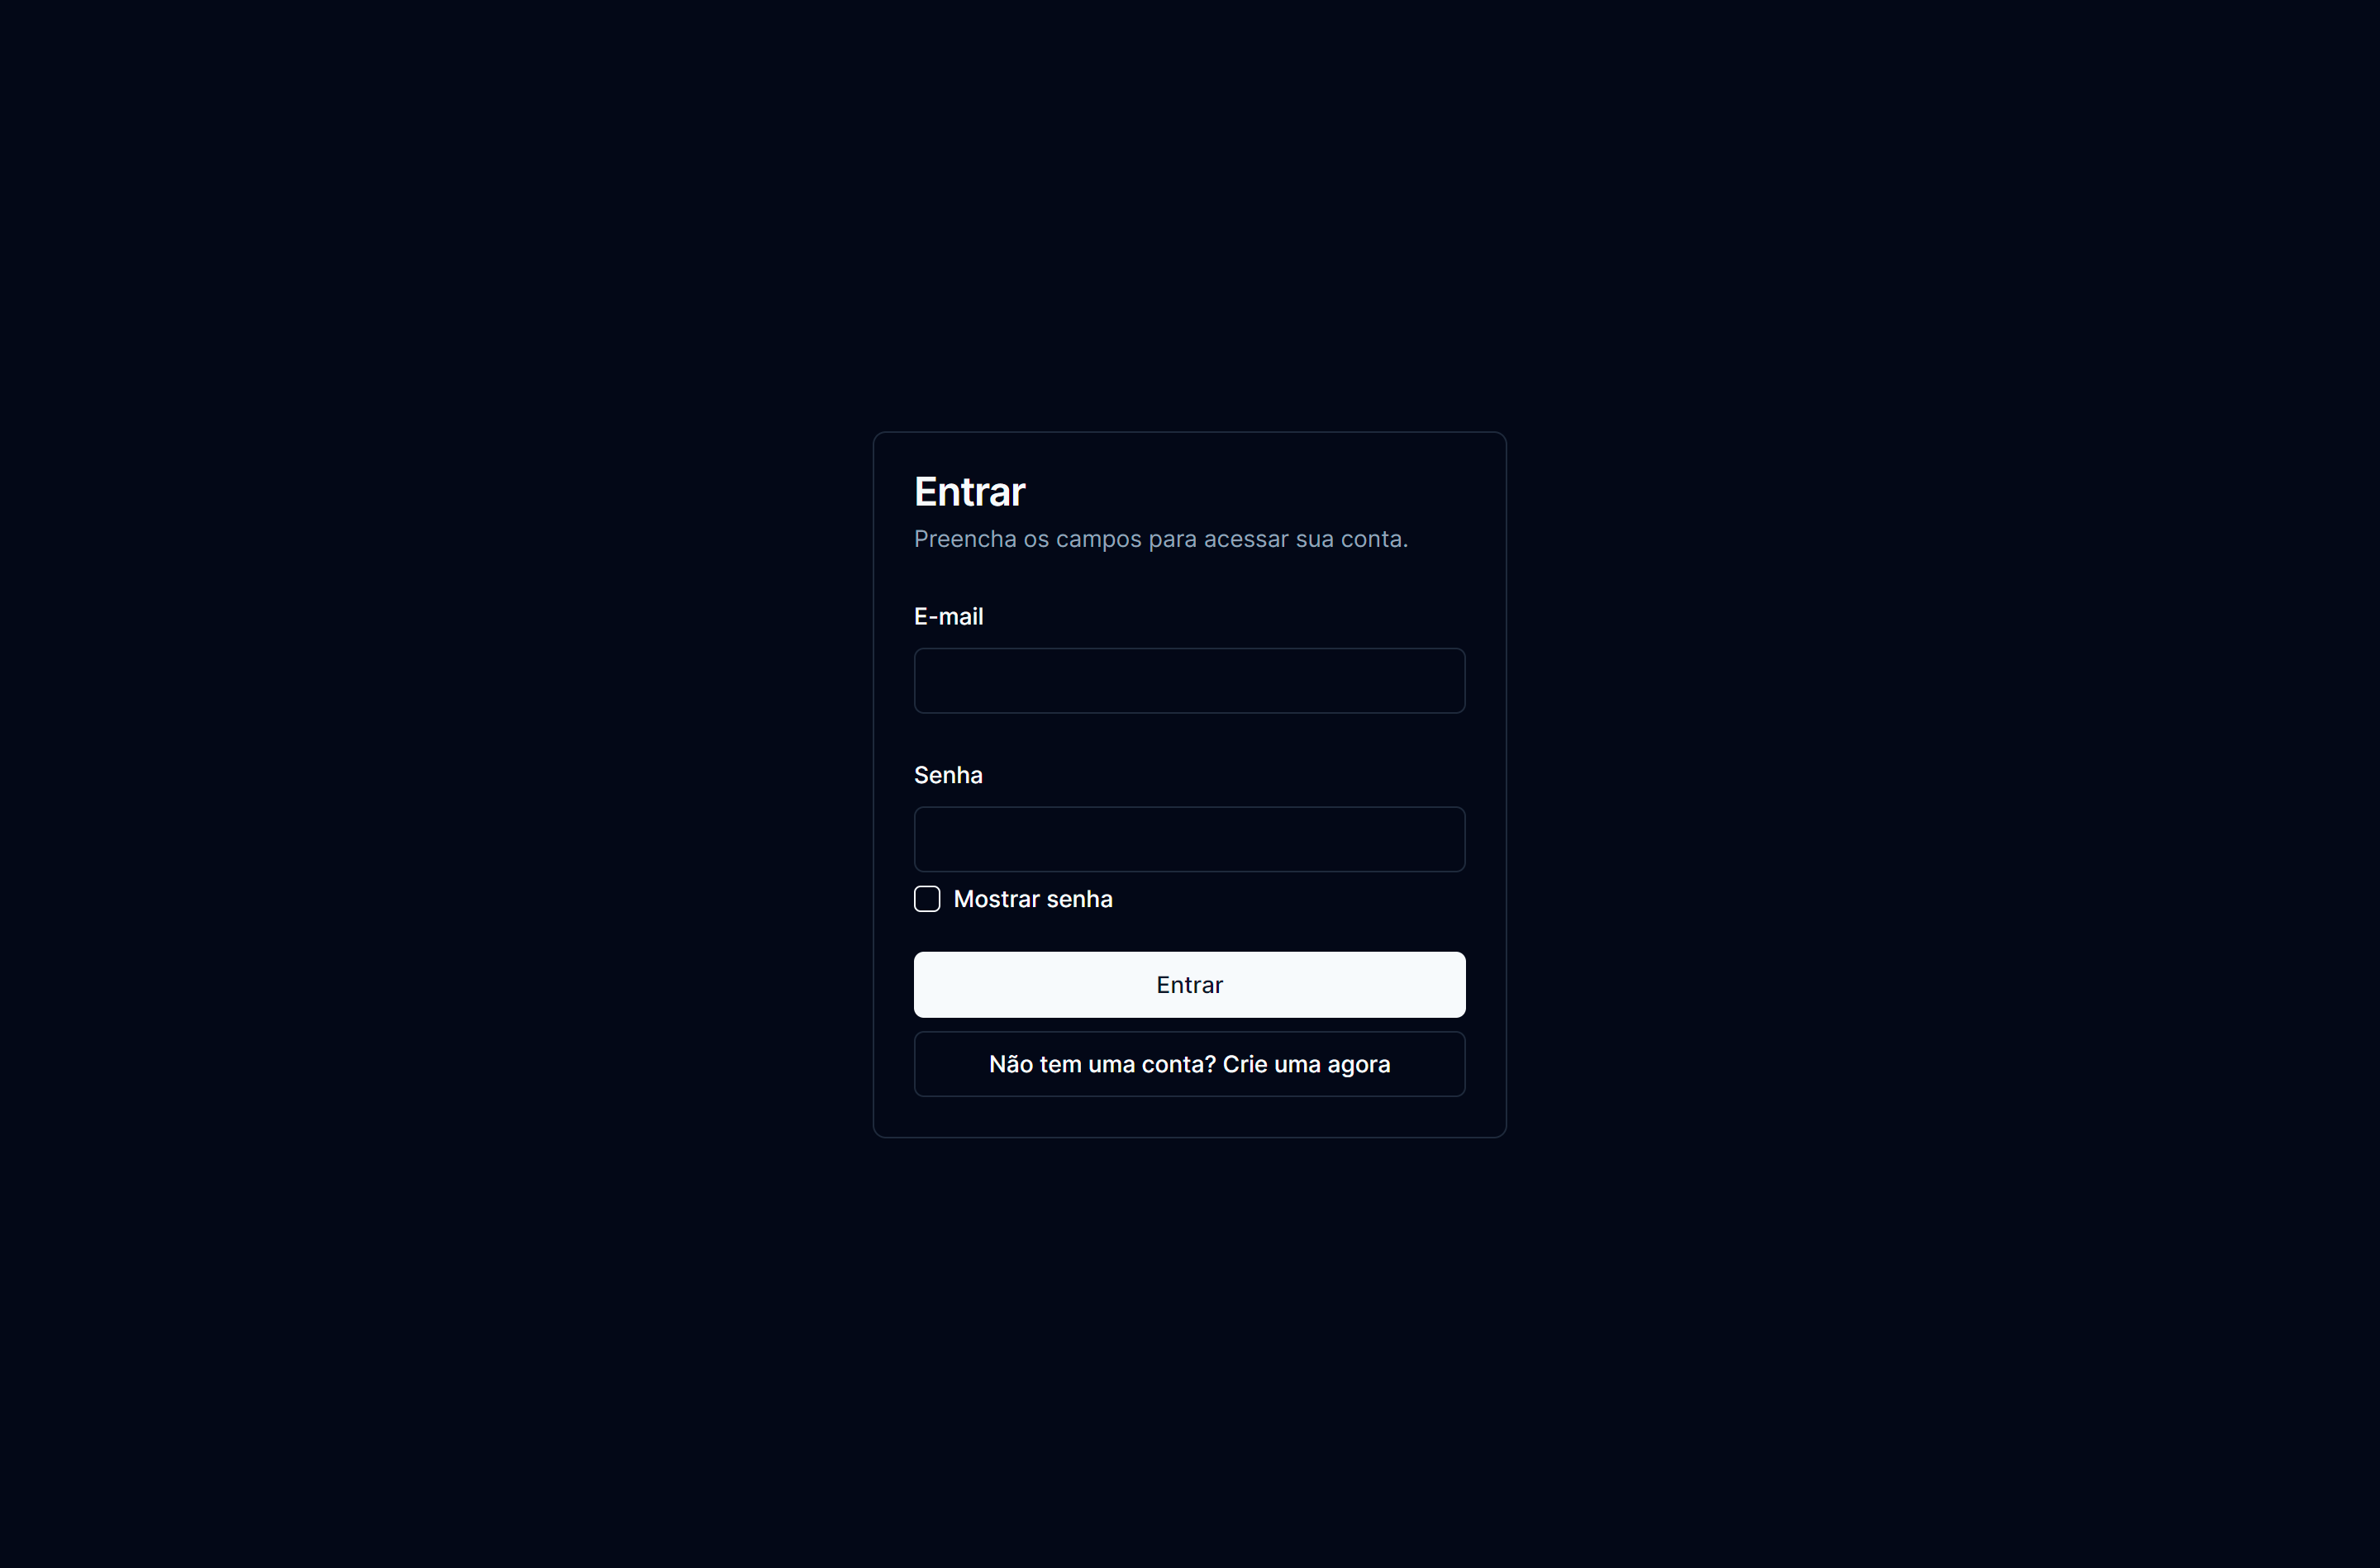
\includegraphics[width=0.8\textwidth]{assets/codeboard/login-page.png}
\end{figure}

\begin{figure}[H]{0.8\textwidth}
    \centering
    \caption{Página de cadastro da plataforma Codeboard UERJ.}
    \label{fig:signup-page}
    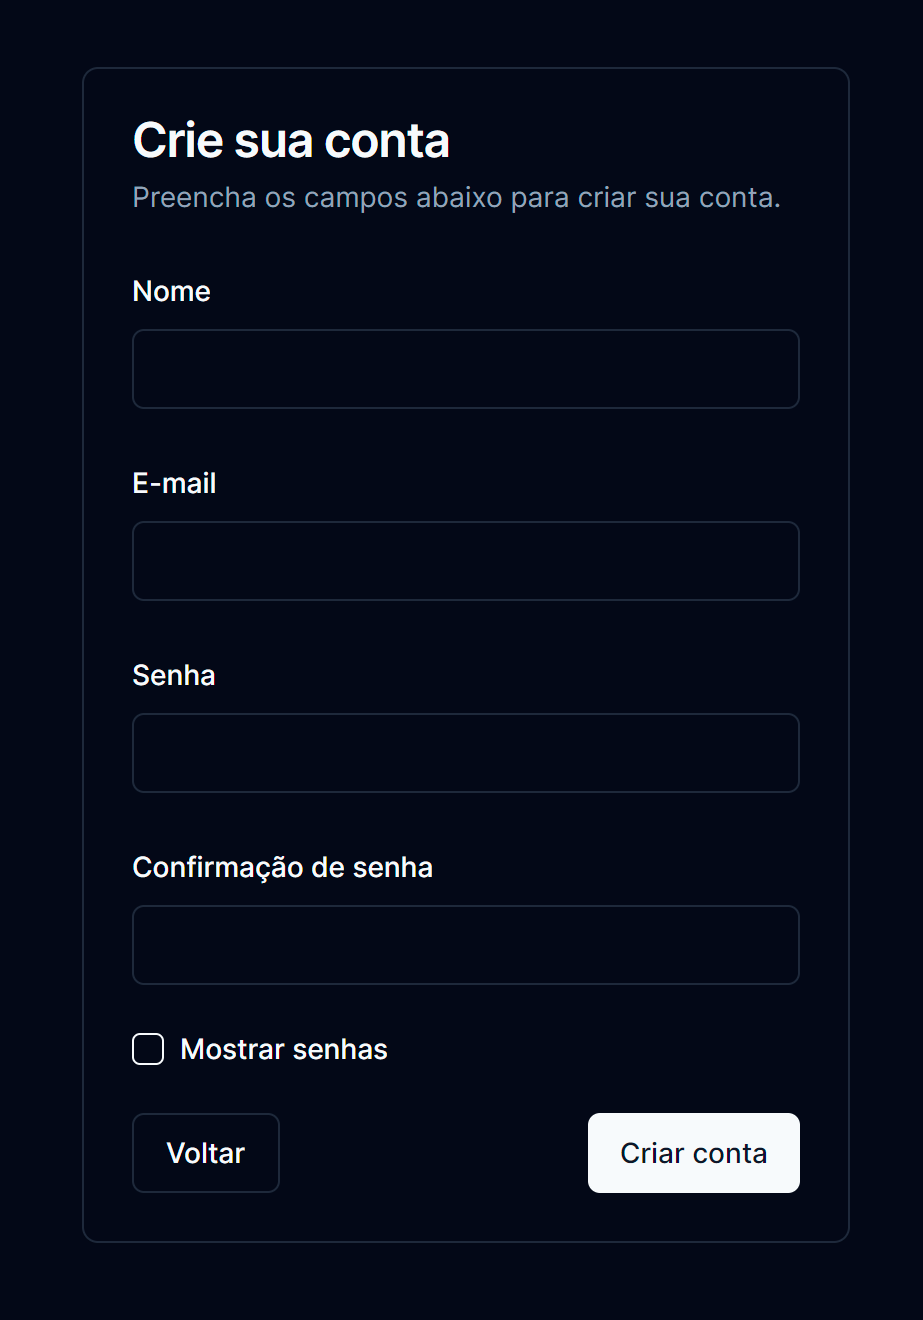
\includegraphics[width=0.8\textwidth]{assets/codeboard/signup-page.png}
\end{figure}

Durante o processo de autenticação, a plataforma utiliza tokens para manter a sessão do usuário ativa. O token é gerado no servidor e enviado ao cliente, sendo armazenado no navegador por meio de cookies. Esse token é então utilizado em todas as requisições subsequentes feitas ao servidor, garantindo que o usuário permaneça autenticado enquanto navega pelas diversas páginas da plataforma.

\subsection{Gerenciamento de Salas}
% Revisado

A funcionalidade de gerenciamento de salas, ilustrada na Figura \ref{fig:rooms-page}, constitui a página inicial da plataforma. Nessa página, as salas são apresentadas em uma lista, onde cada sala é representada por um cartão que exibe o nome, a descrição e o número de participantes. O usuário pode acessar uma sala ao clicar no respectivo cartão, sendo então redirecionado para a tela da sala.

\begin{figure}[H]{1\textwidth}
    \centering
    \caption{Página de listagem de salas da plataforma Codeboard UERJ.}
    \label{fig:rooms-page}
    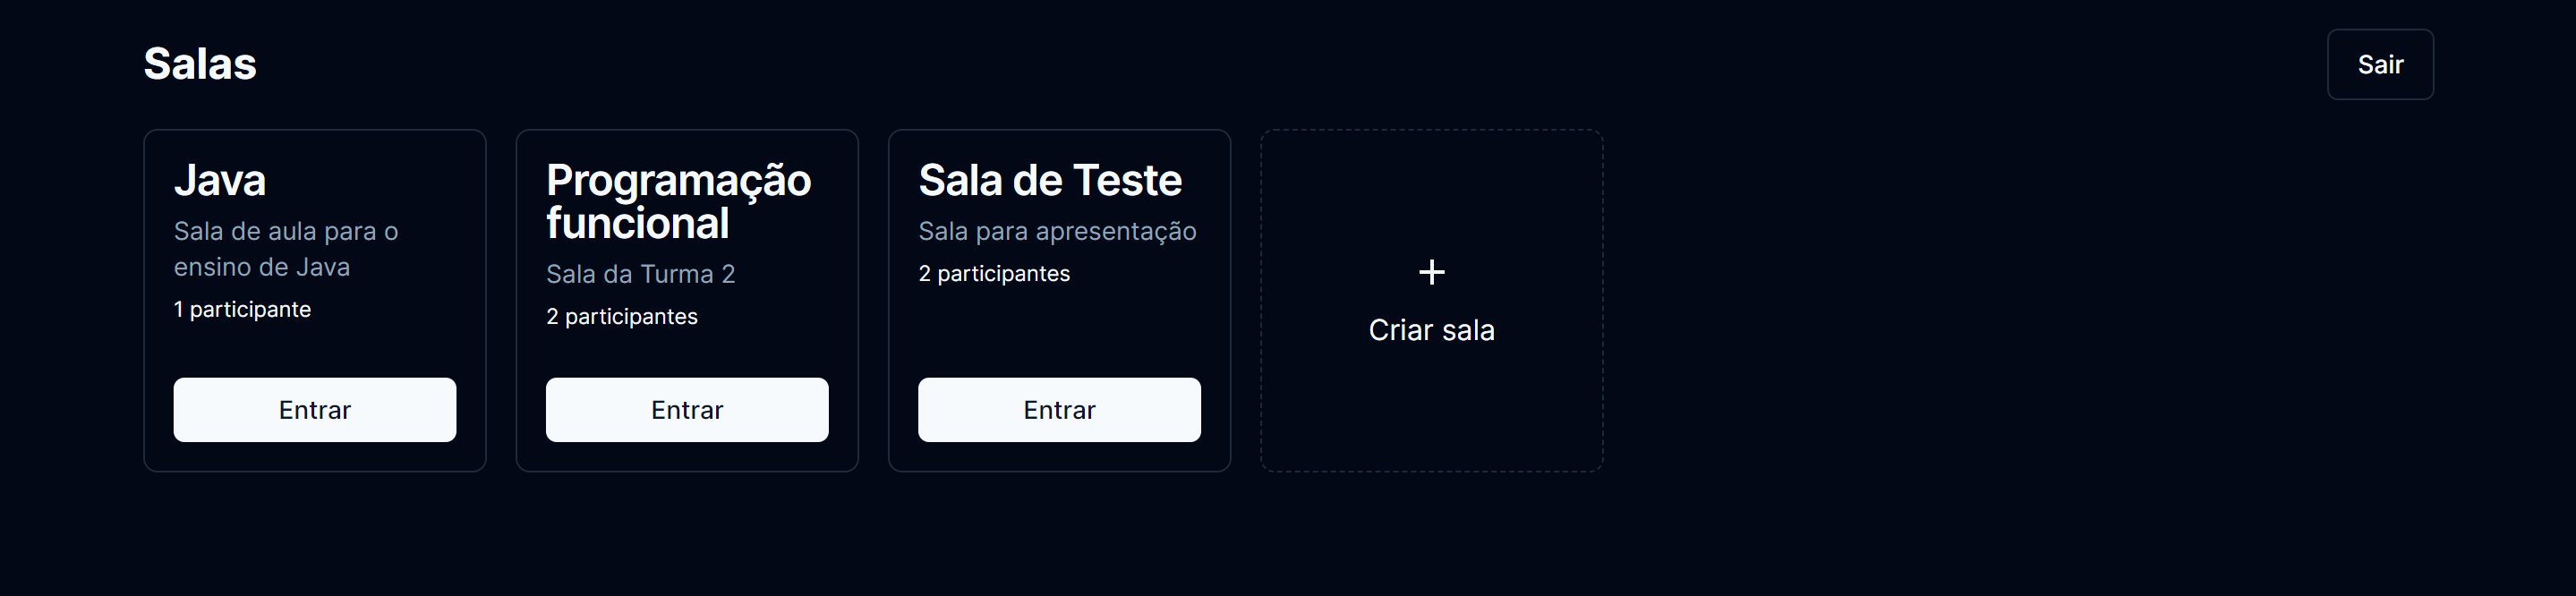
\includegraphics[width=1\textwidth]{assets/codeboard/rooms-page.png}
\end{figure}


Além disso, o usuário pode criar uma nova sala diretamente na tela inicial, utilizando o botão de criação de sala. Ao clicar no botão, o usuário é redirecionado para a página de criação de sala, mostrada na Figura \ref{fig:create-room-page}. Nessa página, é possível inserir o nome e a descrição da sala para concluir a criação.

\begin{figure}[H]{0.75\textwidth}
    \centering
    \caption{Página de criação de sala da plataforma Codeboard UERJ.}
    \label{fig:create-room-page}
    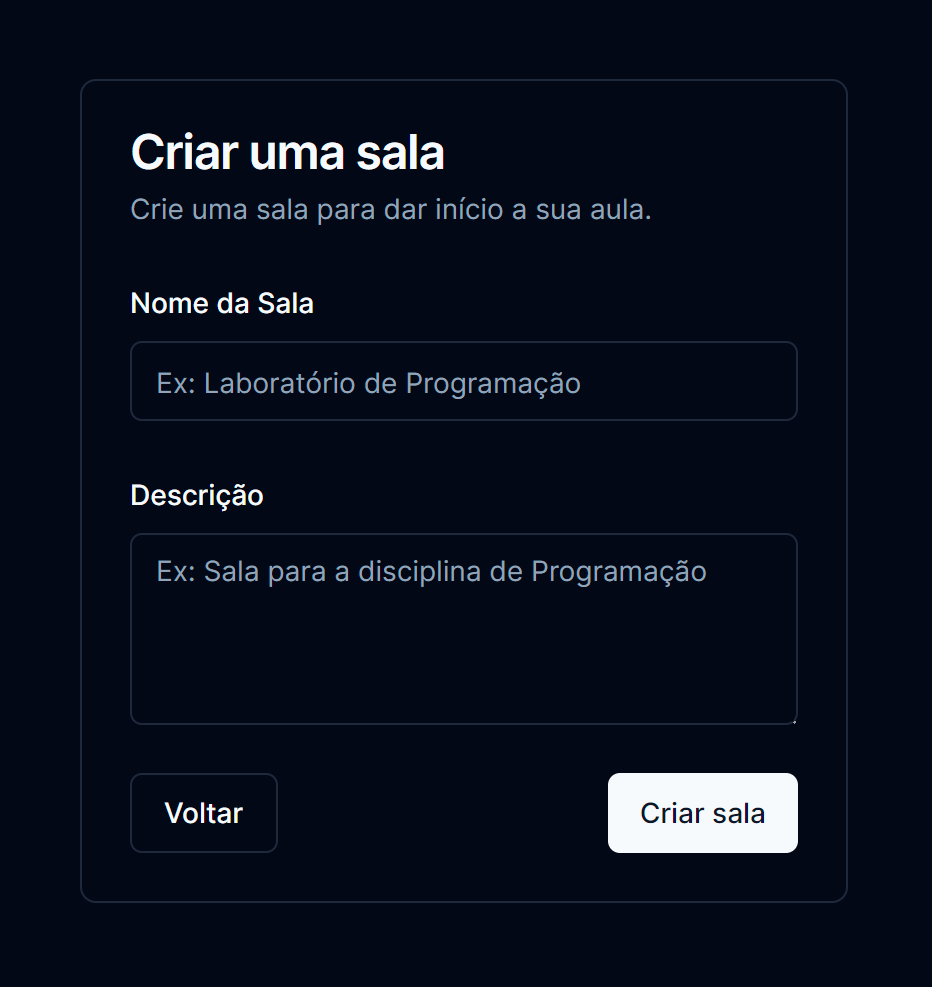
\includegraphics[width=0.75\textwidth]{assets/codeboard/create-room-page.png}
\end{figure}

Após a criação, o usuário é redirecionado para a tela da sala. Para adicionar novos membros, basta clicar no botão de adição de participantes, identificado por um ícone de usuário, conforme mostrado na Figura \ref{fig:add-member-modal}. Uma nova tela será exibida com um campo para inserção do e-mail do aluno que se deseja adicionar à sala. Após a inclusão, o aluno torna-se membro da sala e pode acessá-la.

\begin{figure}[H]{0.8\textwidth}
    \centering
    \caption{Tela de adição de alunos à sala da plataforma Codeboard UERJ.}
    \label{fig:add-member-modal}
    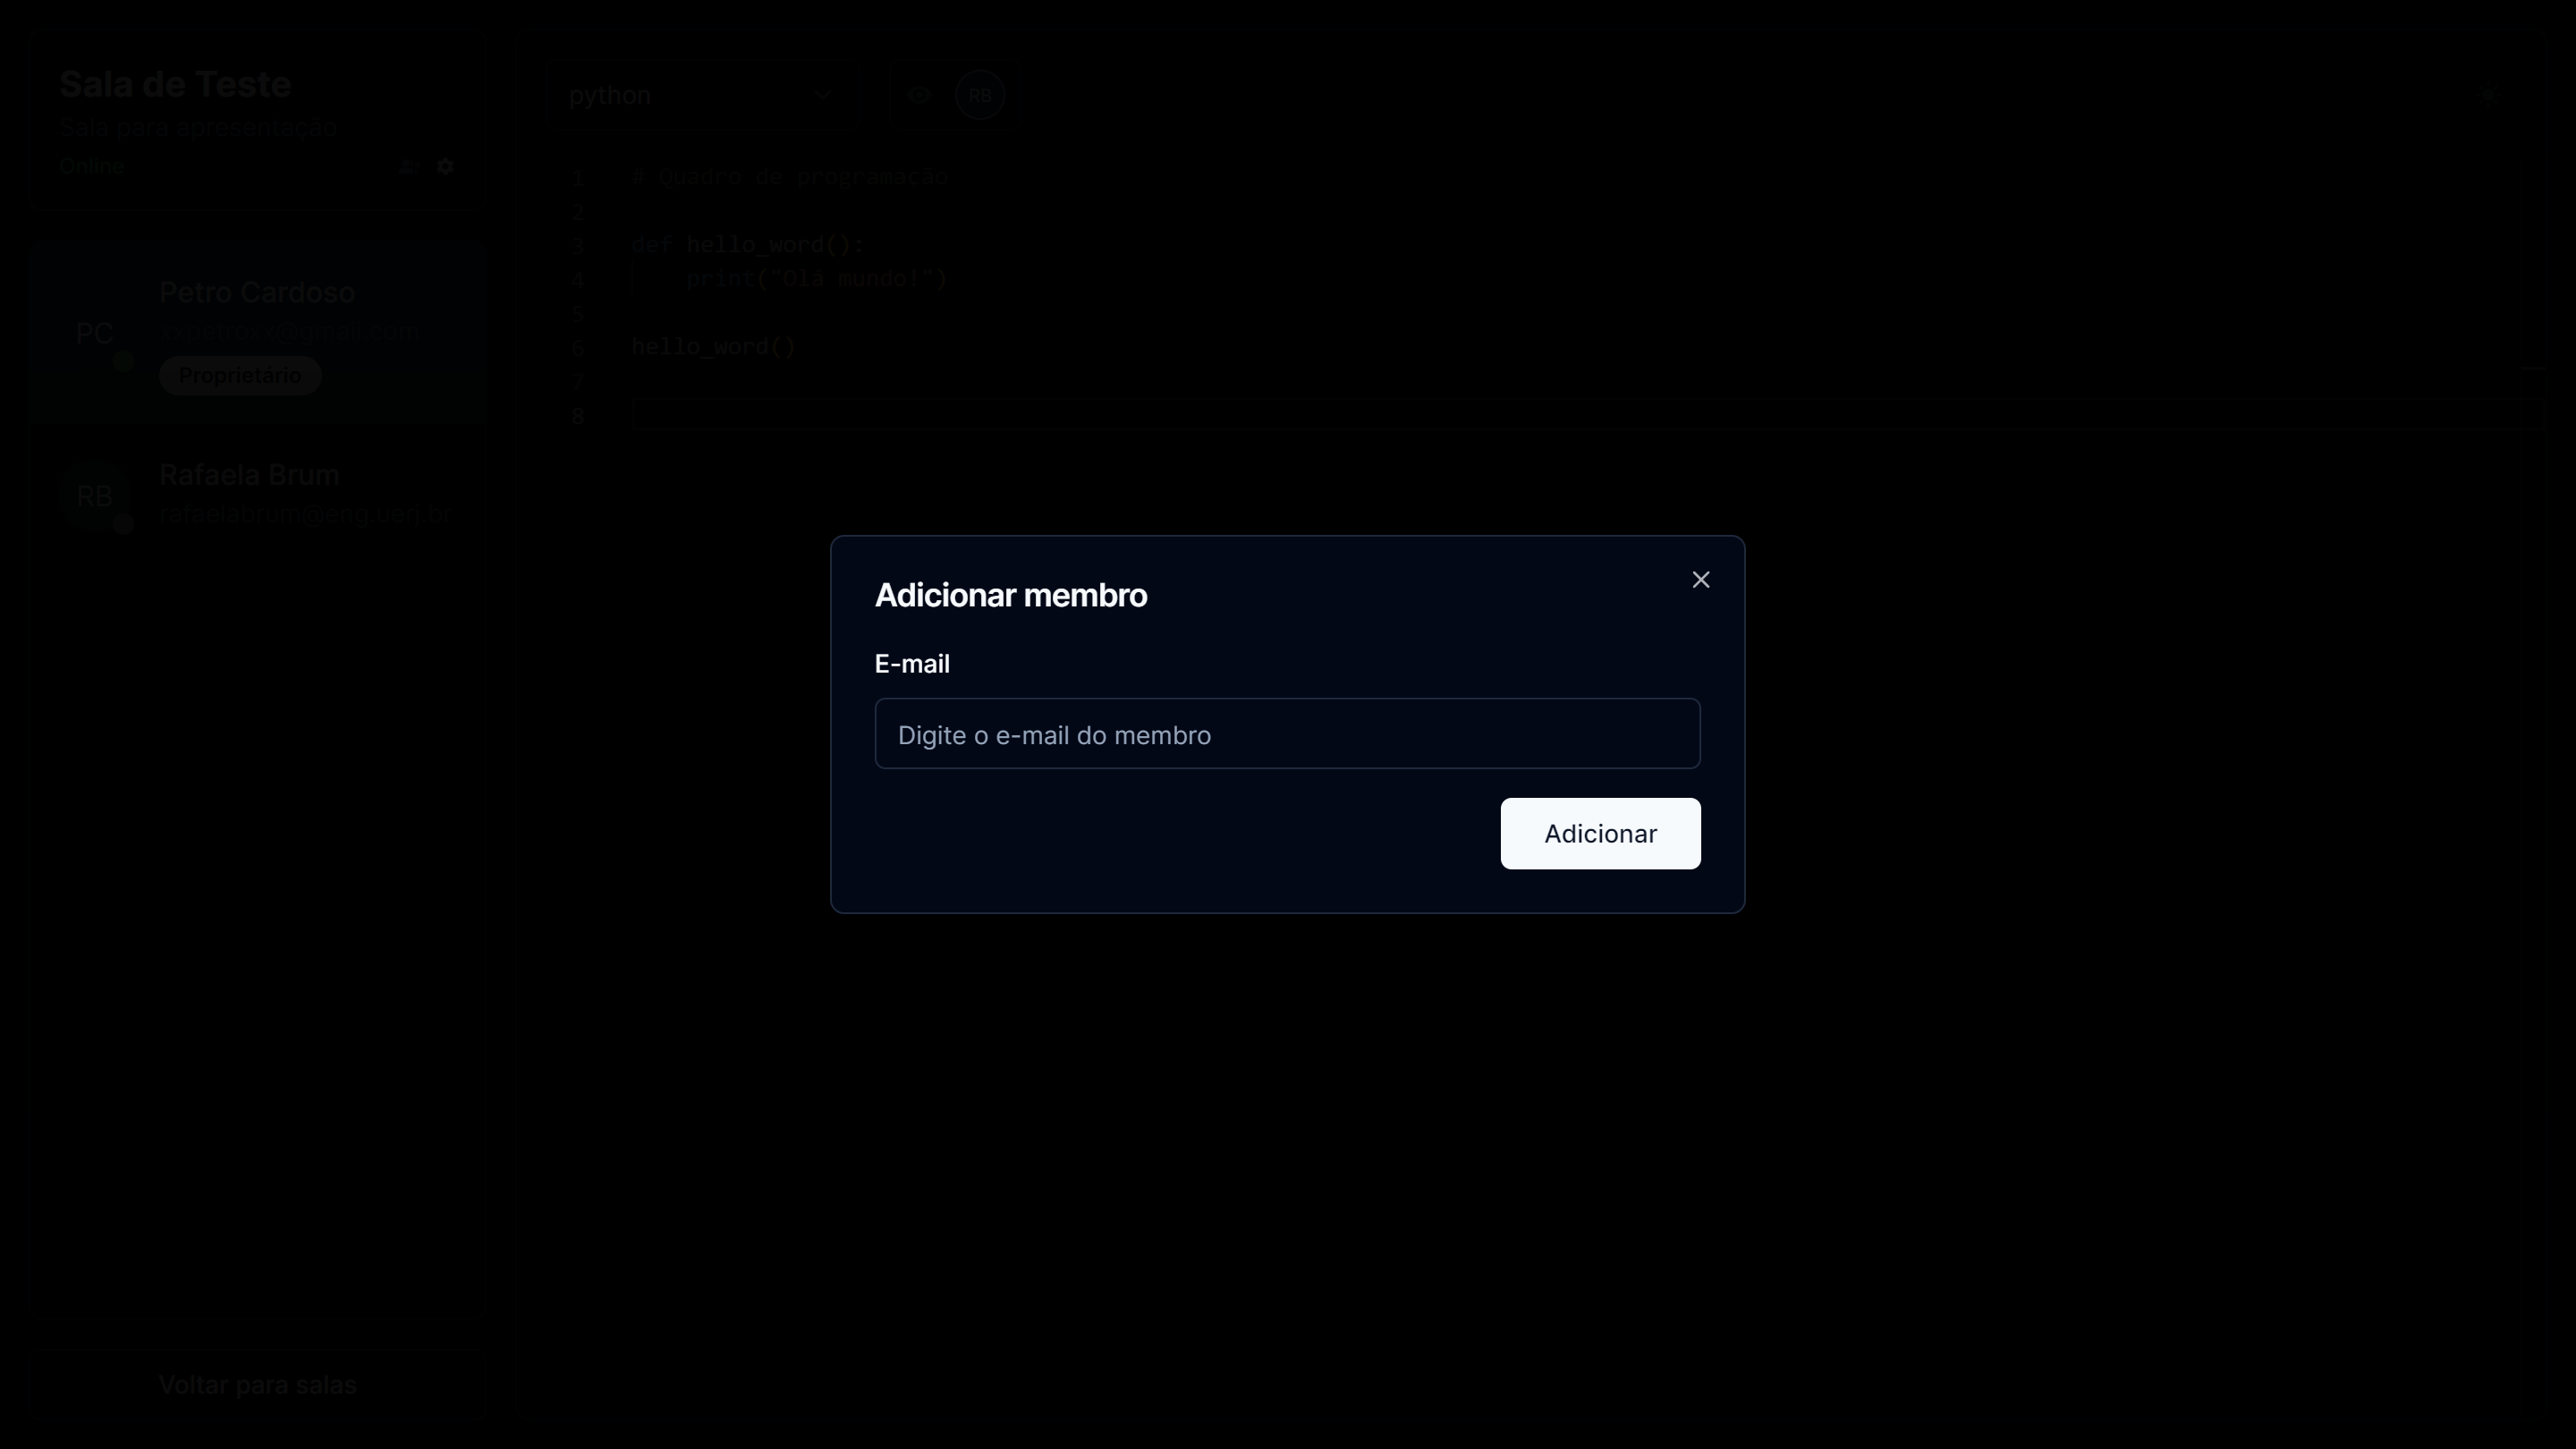
\includegraphics[width=0.8\textwidth]{assets/codeboard/add-member-modal.png}
\end{figure}


O fluxo descrito do gerenciamento de salas está representado no diagrama da Figura \ref{fig:user-room-flow}.


\begin{figure}[H]{0.85\textwidth}
    \centering
    \caption{Diagrama do fluxo de gerenciamento de salas.}
    \label{fig:user-room-flow}
    \includegraphics[width=0.85\textwidth]{diagrams/user-room-flow.png}
\end{figure}

\subsection{Quadro de Programação em Tempo Real}
% Revisado

A principal funcionalidade da plataforma é o quadro de programação em tempo real, que permite aos alunos escreverem códigos diretamente no navegador, sem a necessidade de instalar um ambiente de desenvolvimento integrado (IDE).

Para acessar o quadro de programação, o usuário deve entrar na sala desejada por meio da página de gerenciamento de salas. A plataforma exibe uma tela dividida em dois módulos: o módulo lateral, que contém a seleção de usuários, e o módulo central, onde ocorre a edição de código.

\begin{figure}[H]{1\textwidth}
    \centering
    \caption{Página da sala de programação da plataforma Codeboard UERJ.}
    \label{fig:room-details-page}
    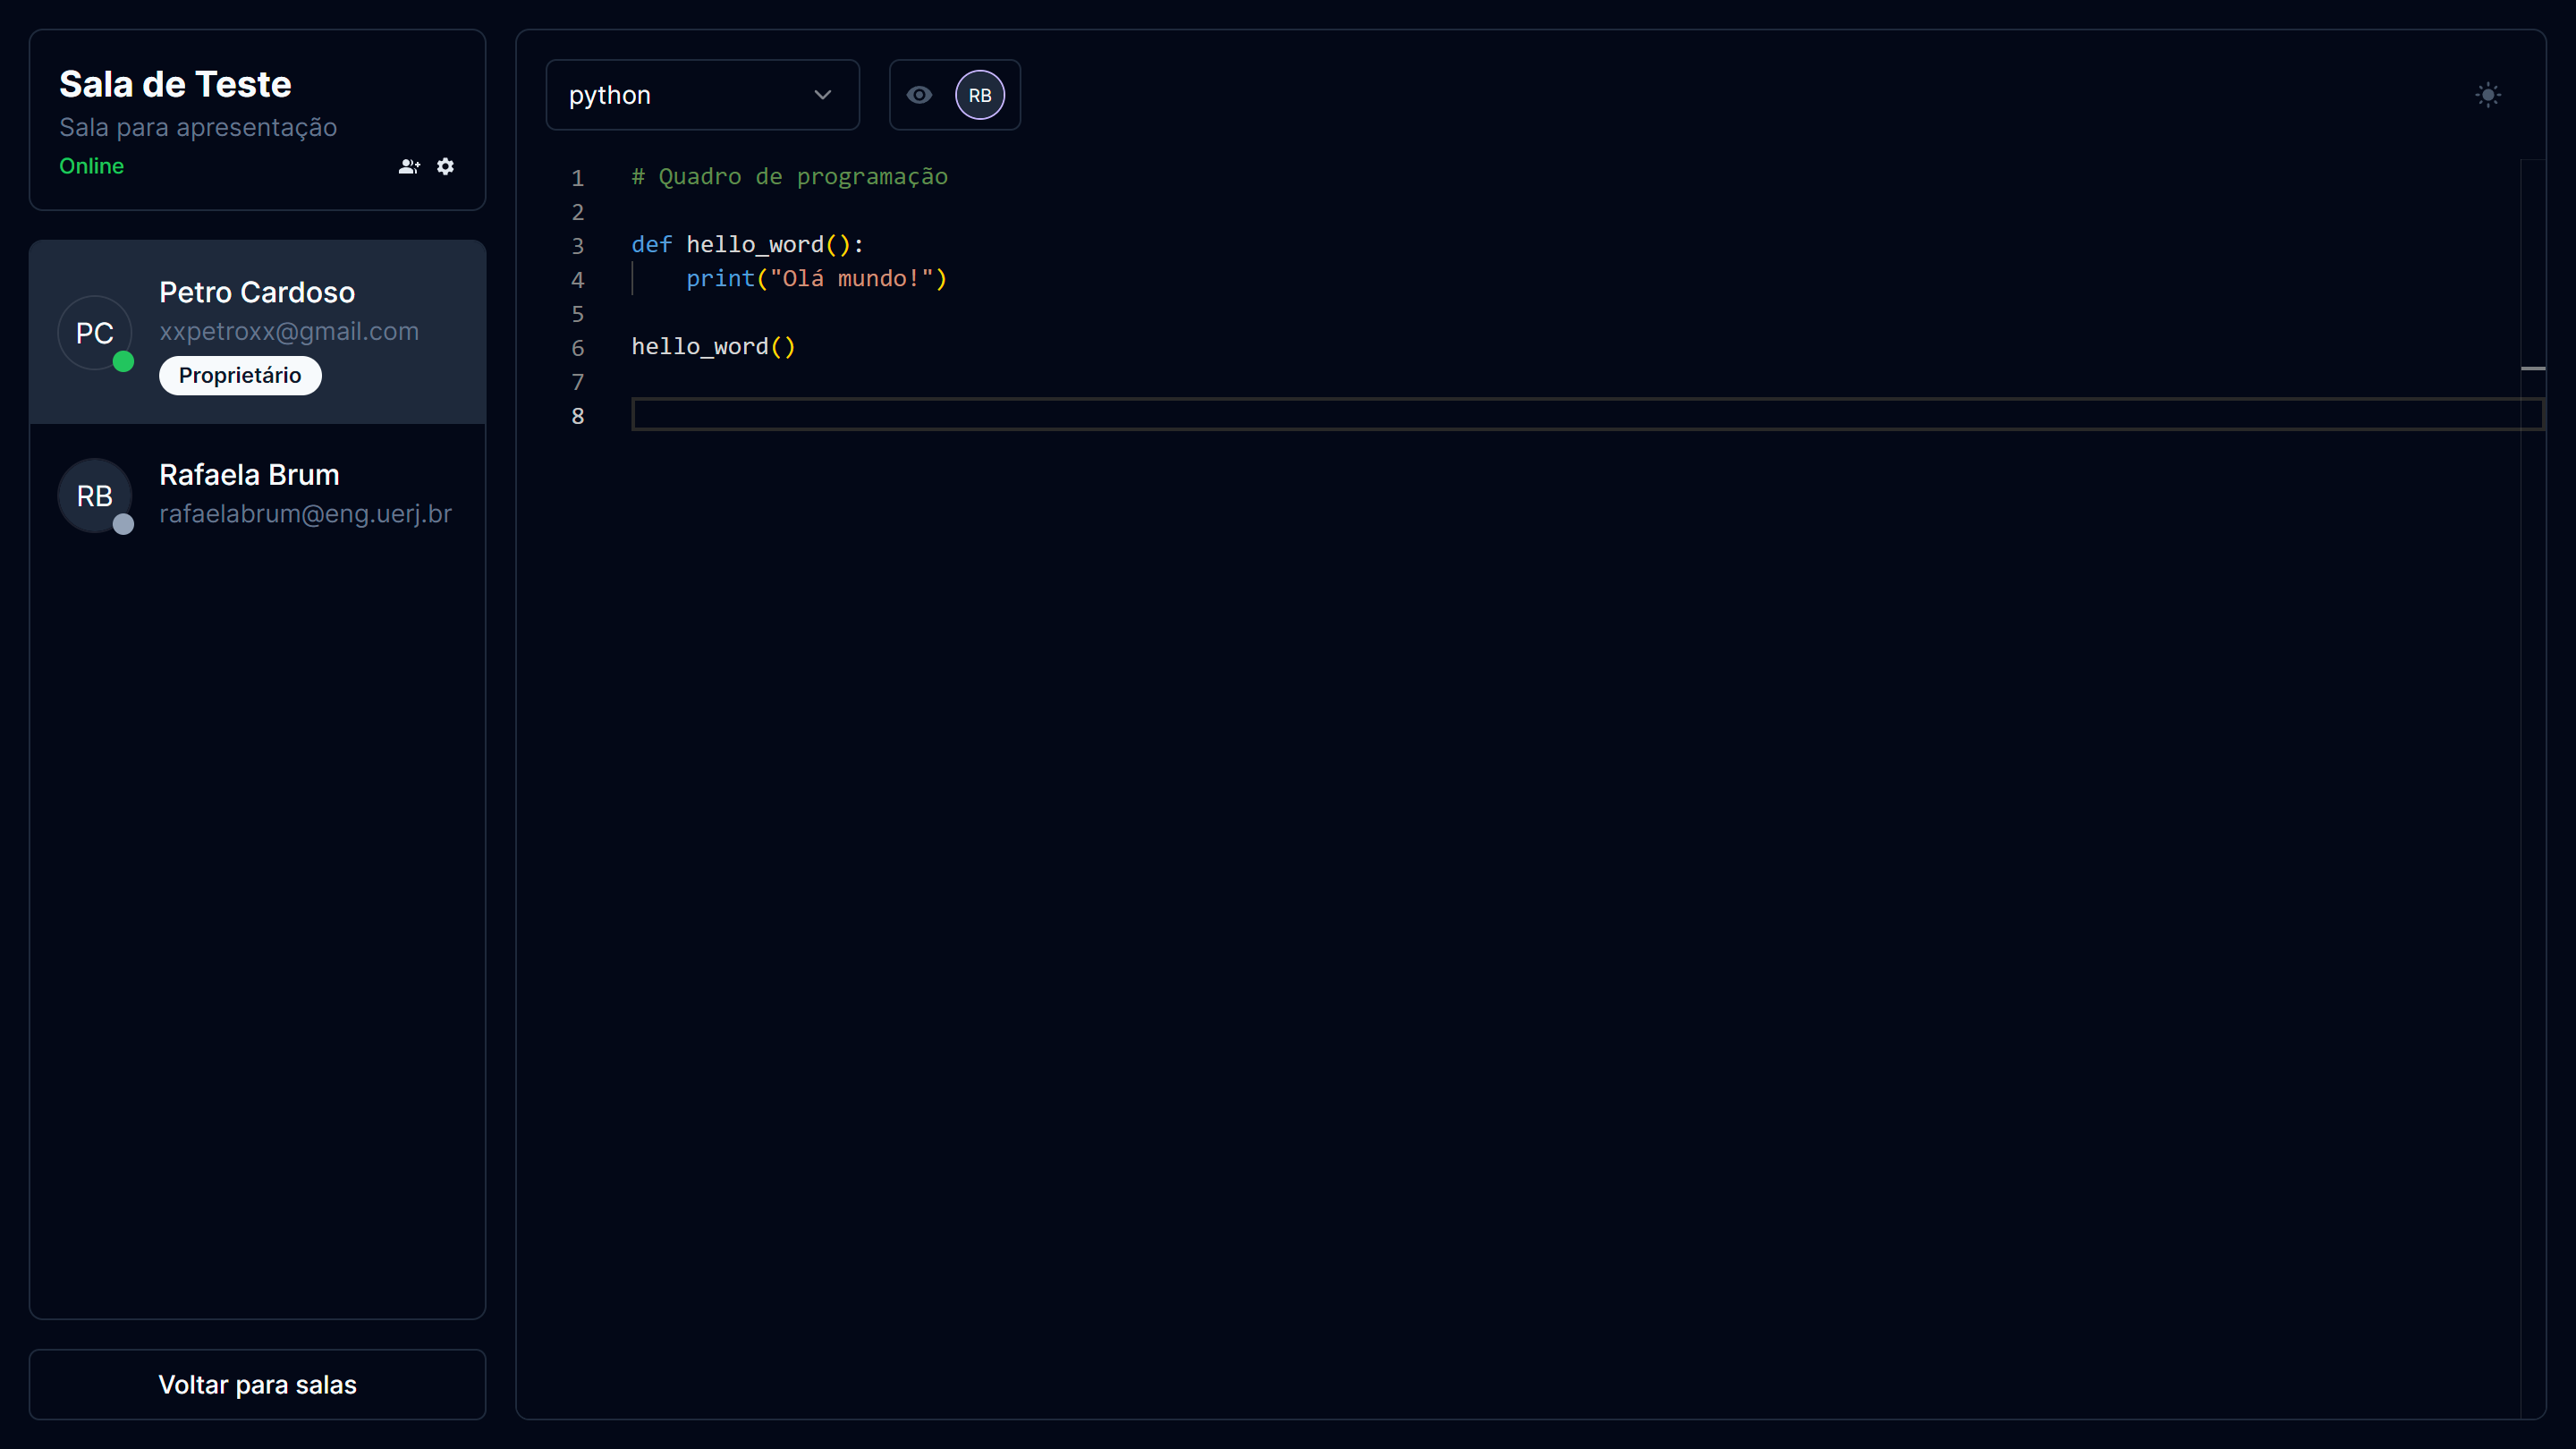
\includegraphics[width=1\textwidth]{assets/codeboard/room-details-page.png}
\end{figure}

Como mostrado na Figura \ref{fig:room-details-page}, o módulo lateral exibe a lista de participantes da sala, onde são apresentados o nome, a foto de perfil e indicadores que informam se o participante está online ou editando seu código. O usuário pode selecionar outro membro da sala para visualizar e interagir com o código dele em tempo real.

Caso o usuário selecione a si mesmo, ele poderá editar o próprio código, mudar a linguagem de programação e visualizar quem está acessando seu código. As edições são salvas automaticamente a cada modificação.

Acima do módulo lateral, o nome e a descrição da sala são exibidos. Se o usuário for o proprietário da sala, ele também verá os botões de adição de participantes e de configuração da sala. O botão de adição permite convidar novos membros, enquanto o botão de configuração possibilita a edição do nome e da descrição da sala. As figuras \ref{fig:add-member-modal} e \ref{fig:edit-room-modal} mostram os modais de adição de participantes e de configuração de sala, respectivamente.

\begin{figure}[H]{0.8\textwidth}
    \centering
    \caption{Modal de configuração de sala da plataforma Codeboard UERJ.}
    \label{fig:edit-room-modal}
    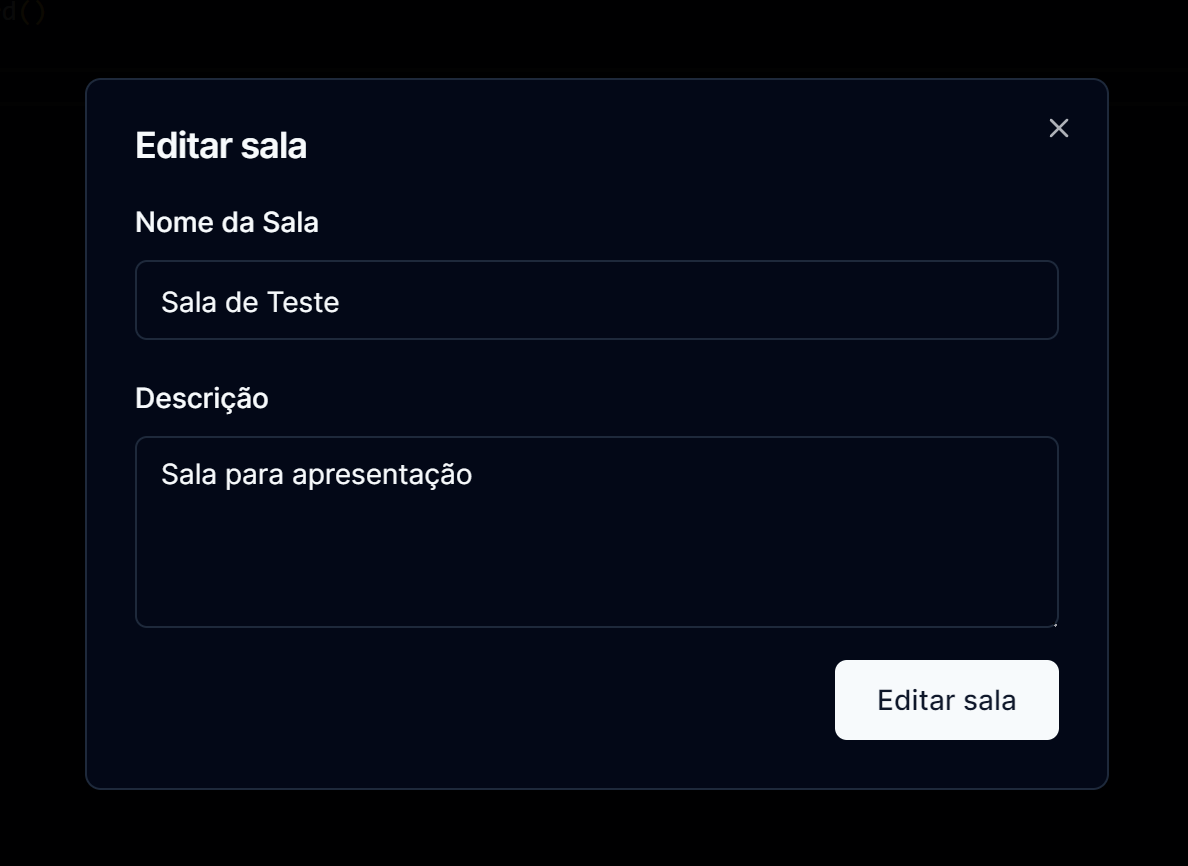
\includegraphics[width=0.8\textwidth]{assets/codeboard/edit-room-modal.png}
\end{figure}

Na parte inferior do módulo lateral, encontra-se o botão de saída, que redireciona o usuário de volta para a página de listagem de salas, onde ele pode acessar outras salas ou criar novas.

O módulo central abriga o editor de código, que oferece funcionalidades típicas de uma IDE, como coloração de sintaxe, auto-completar e formatação de código. Quando o usuário está visualizando o código de outro participante, ele pode fazer marcações visíveis em tempo real para todos os membros da sala, facilitando a comunicação e a colaboração. A Figura \ref{fig:code-editor-user-highlight} mostra um exemplo de marcação de código na plataforma.

\begin{figure}[H]{0.85\textwidth}
    \centering
    \caption{Marcação de código na plataforma Codeboard UERJ.}
    \label{fig:code-editor-user-highlight}
    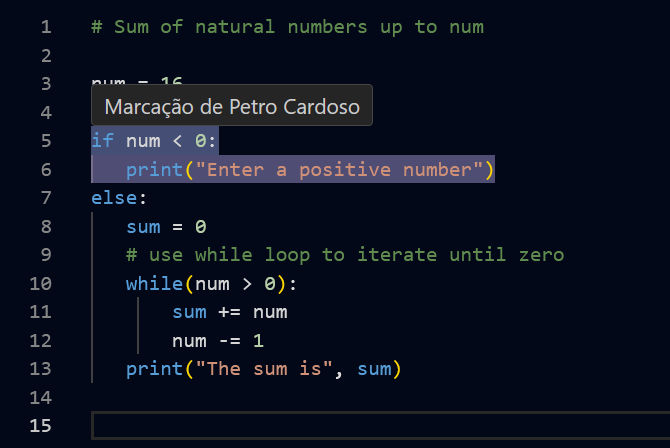
\includegraphics[width=0.85\textwidth]{assets/codeboard/code-editor-user-highlight.png}
\end{figure}

Na parte superior do editor, é possível selecionar a linguagem de programação desejada, com suporte para as linguagens mais utilizadas, como C, C++, Java, Python, Javascript etc. A escolha da linguagem altera a coloração de sintaxe, facilitando tanto a escrita quanto a leitura do código. 

Ao lado da seleção de linguagem, a plataforma exibe uma lista horizontal de quem está visualizando o código no momento, permitindo ao usuário monitorar em tempo real quem acompanha seu progresso.

A Figura \ref{fig:code-editor-toolbar} mostra a barra de ferramentas do editor de código, onde estão localizados os botões para seleção da linguagem de programação e para visualização dos usuários que estão acompanhando o quadro em tempo real.

\begin{figure}[H]{0.8\textwidth}
    \centering
    \caption{Barra de ferramentas do editor de código da plataforma.}
    \label{fig:code-editor-toolbar}
    
\includegraphics[width=0.8\textwidth]{assets/codeboard/code-editor-toolbar.png}
\end{figure}


\subsection{Regras de Negócio}

Existem algumas regras de negócio que devem ser seguidas para garantir o bom funcionamento da plataforma. Estas regras são implementadas no backend da plataforma e são responsáveis por validar os dados dos usuários e das salas, bem como garantir a segurança e a integridade dos dados.

\paragraph{Autenticação}

\begin{itemize}
    \item \textbf{Cadastro de Usuários}: A plataforma deve fornecer um mecanismo de registro que permita aos usuários criarem suas contas. Durante esse processo, serão solicitados dados como nome, e-mail e senha, que devem ser armazenados com segurança no banco de dados.
    \item \textbf{Validação de Dados}: É essencial que a plataforma assegure a qualidade e integridade das informações fornecidas pelos usuários. Isso inclui verificar a consistência dos dados durante o cadastro e o login, garantindo que apenas entradas válidas sejam aceitas.
    \item \textbf{Proteção de Dados}: Para resguardar as informações dos usuários, a plataforma deve aplicar técnicas de criptografia e hashing no armazenamento de dados sensíveis, prevenindo acessos não autorizados.
    \item \textbf{Login de Usuários}: O sistema de login deve verificar as credenciais informadas, como e-mail e senha, permitindo acesso apenas a usuários previamente cadastrados. Após a autenticação bem-sucedida, será gerado um token para manter a sessão ativa.
    \item \textbf{Gerenciamento de Sessões}: É fundamental administrar as sessões de forma eficiente, utilizando tokens de autenticação para identificar os usuários e encerrando sessões automaticamente após períodos prolongados de inatividade.
    \item \textbf{Restrição de Acesso}: Para proteger as funcionalidades da plataforma, o acesso deve ser limitado a usuários autenticados. A verificação da autenticação será realizada antes de liberar qualquer recurso ou serviço.
\end{itemize}

\paragraph{Gerenciamento de Salas}

\begin{itemize}
    \item \textbf{Criação de Salas}: A plataforma deve permitir que os usuários criem novas salas fornecendo informações como nome e descrição. Esses dados devem ser armazenados de forma segura no banco de dados.
    \item \textbf{Validação de Dados}: Para assegurar a integridade das informações, os dados das salas devem ser verificados durante os processos de criação e edição, garantindo consistência e validade.
    \item \textbf{Restrição de Acesso}: O acesso às salas será concedido apenas a participantes autorizados, com a confirmação de que o usuário é dono ou membro da sala antes de permitir a entrada.
    \item \textbf{Gerenciamento de Participantes}: Apenas usuários com permissões administrativas, como os proprietários das salas, poderão adicionar ou remover participantes.
    \item \textbf{Restrição de Edição}: A edição das informações da sala será limitada exclusivamente ao proprietário, mediante validação da propriedade antes de qualquer alteração.
\end{itemize}

\paragraph{Quadro de Programação}

\begin{itemize}
    \item \textbf{Editor em Tempo Real}: A plataforma deve disponibilizar um editor de código em tempo real, permitindo que os usuários programem diretamente no navegador. O editor deve incluir funcionalidades típicas de um IDE, como coloração de sintaxe, auto-completar e formatação de código.
    \item \textbf{Restrição de Escrita}: Conflitos durante a edição colaborativa serão evitados ao permitir que apenas o proprietário do código realize alterações, utilizando um mecanismo que bloqueia a escrita para os demais participantes
    \item \textbf{Marcação de Código}: O sistema deve possibilitar o destaque de trechos de código em tempo real, permitindo que os usuários acompanhem e interajam com as edições feitas por outros colaboradores no quadro.
    \item \textbf{Seleção de Linguagem}: A plataforma deve permitir a escolha da linguagem de programação diretamente no editor, ajustando automaticamente a coloração de sintaxe para a linguagem selecionada.
    \item \textbf{Visualização de Usuários}: Os usuários devem ter acesso a uma lista que mostre, em tempo real, quem está visualizando ou interagindo com o código no quadro.
\end{itemize}

\paragraph{Lista de Participantes}

\begin{itemize}
    \item \textbf{Visualização de Participantes}: A plataforma deve exibir uma lista que informe aos usuários quem está presente na sala, facilitando a identificação dos participantes ativos.
    \item \textbf{Indicadores de Presença}: Os usuários devem ter acesso a indicadores que mostrem quem está online e quem está editando o código no momento, tornando a colaboração mais clara e eficiente.
    \item \textbf{Seleção de Participantes}: Será possível selecionar participantes específicos para visualizar e interagir com o código deles, utilizando uma interface que permita essa escolha de forma simples e intuitiva.
\end{itemize}


\section{Implementação}
% Revisado

Nesta seção, será apresentada a implementação da plataforma Codeboard UERJ. A plataforma é estruturada em três componentes principais: o backend, o banco de dados e o frontend. Cada um deles desempenha um papel específico na plataforma, sendo responsável pelas regras de negócio, o armazenamento de dados e a interface com o usuário, respectivamente.

\subsection{Backend}
% Revisado

O backend da plataforma é responsável pela implementação das regras de negócio da aplicação. Ele é composto por um servidor NodeJS que utiliza dois métodos de comunicação: REST API e WebSockets. A REST API é usada para comunicação assíncrona entre o cliente e o servidor, enquanto os WebSockets são utilizados para permitir a comunicação em tempo real entre os usuários.

A comunicação entre o cliente e o servidor ocorre através de duas interfaces principais: REST API e WebSockets. A REST API fornece um conjunto de rotas que permitem ao cliente acessar funcionalidades da plataforma, como autenticação de usuários, gerenciamento de salas e edição de código. Os WebSockets, por sua vez, são utilizados para viabilizar a comunicação em tempo real entre os usuários, possibilitando a edição colaborativa de código. A Figura \ref{fig:backend-architecture} ilustra a arquitetura do backend da plataforma Codeboard UERJ.

\begin{figure}[H]{0.8\textwidth}
    \centering
    \caption{Arquitetura do backend da plataforma Codeboard UERJ.}
    \label{fig:backend-architecture}
    \includegraphics[width=0.75\textwidth]{diagrams/backend-architecture.png}
\end{figure}


\subsection{Banco de Dados NoSQL}
% Revisado

A plataforma utiliza o MongoDB, um banco de dados NoSQL orientado a documentos, devido à sua flexibilidade, escalabilidade horizontal e eficiência no armazenamento de grandes volumes de dados. Além disso, a integração simples com o NodeJS fez do MongoDB uma escolha natural para a plataforma Codeboard UERJ.

O banco de dados é estruturado em três coleções principais: a coleção de usuários (Users), a de salas (Rooms) e a de quadros de programação (Board). Essa organização está diretamente ligada às funcionalidades da plataforma, proporcionando armazenamento e recuperação eficazes dos dados dos usuários, das salas e dos quadros de programação. A Figura \ref{fig:database-schema} ilustra como essas coleções estão organizadas e como se relacionam no banco de dados.

\begin{figure}[H]{0.75\textwidth}
    \centering
    \caption{Esquema do banco de dados da plataforma.}
    \label{fig:database-schema}
    \includegraphics[width=0.75\textwidth]{diagrams/database-schema.png}
\end{figure}

A coleção de usuários armazena dados como nome, e-mail e senha dos usuários cadastrados. A Tabela \ref{tab:user-collection-fields} detalha os campos dessa coleção, que inclui:

\begin{itemize}
    \item \textbf{\_id}: Identificador único do usuário.
    \item \textbf{name}: Nome do usuário.
    \item \textbf{email}: E-mail do usuário.
    \item \textbf{password}: Hash da senha do usuário.
    \item \textbf{createdAt}: Data de criação do usuário.
\end{itemize}

\begin{table}[H]{1\textwidth}
    \centering
    \caption{Campos da coleção "User" do banco de dados da plataforma Codeboard UERJ.}
    \label{tab:user-collection-fields}
    \renewcommand{\arraystretch}{1.3} 
    \begin{tabular}{|c|c|c|c|}
        \hline
        \textbf{Campo}   & \textbf{Tipo} & \textbf{Obrigatório} \\
        \hline
        \_id            & ObjectId      & Sim                  \\
        \hline
        name              & String        & Sim                  \\
        \hline
        email              & String        & Sim                  \\
        \hline
        password         & String        & Sim                  \\
        \hline
        createdAt        & Date          & Sim                  \\
        \hline
    \end{tabular}
\end{table}

A coleção de usuários possui um campo password que armazena o hash da senha do usuário em vez da senha em texto puro. Essa prática garante a segurança dos dados, evitando que as senhas sejam armazenadas de forma insegura, o que poderia comprometer os usuários em caso de vazamento de informações.


A coleção de salas contém informações sobre as salas criadas, como nome, descrição e participantes. A Tabela \ref{tab:room-collection-fields} apresenta os campos dessa coleção, incluindo:

\begin{itemize}
    \item \textbf{\_id}: Identificador único da sala.
    \item \textbf{name}: Nome da sala.
    \item \textbf{description}: Descrição da sala.
    \item \textbf{owner}: Identificador do dono da sala.
    \item \textbf{members}: Lista de participantes da sala.
    \item \textbf{createdAt}: Data de criação da sala.
\end{itemize}

\begin{table}[H]{1\textwidth}
    \centering
    \caption{Campos da coleção "Room" do banco de dados da plataforma Codeboard UERJ.}
    \label{tab:room-collection-fields}
    \renewcommand{\arraystretch}{1.3} 
    \begin{tabular}{|c|c|c|c|}
        \hline
        \textbf{Campo}              & \textbf{Tipo}   & \textbf{Obrigatório} \\
        \hline
        \_id              & ObjectId        & Sim                  \\
        \hline
        name                          & String          & Sim                  \\
        \hline
        description               & String          & Não                  \\
        \hline
        owner          & ObjectId        & Sim                  \\
        \hline
        members        & Array<ObjectId> & Não                  \\
        \hline
        createdAt           & Date            & Sim                  \\
        \hline
    \end{tabular}
\end{table}


A coleção de quadros de programação armazena os códigos escritos pelos usuários, juntamente com a linguagem de programação utilizada. A Tabela \ref{tab:board-collection-fields} descreve os campos dessa coleção, que incluem:

\begin{itemize}
    \item \textbf{\_id}: Identificador único do quadro.
    \item \textbf{user}: Identificador do usuário dono do quadro.
    \item \textbf{room}: Identificador da sala do quadro.
    \item \textbf{language}: Linguagem de programação.
    \item \textbf{content}: Código de programação.
    \item \textbf{updatedAt}: Data da última atualização.
    \item \textbf{createdAt}: Data de criação.
\end{itemize}

\begin{table}[H]{1\textwidth}
    \centering
    \caption{Campos da coleção "Board" do banco de dados da plataforma Codeboard UERJ.}
    \label{tab:board-collection-fields}
    \renewcommand{\arraystretch}{1.3} 
    \begin{tabular}{|c|c|c|c|}
        \hline
        \textbf{Campo}             & \textbf{Tipo} & \textbf{Obrigatório} \\
        \hline
        \_id             & ObjectId      & Sim                  \\
        \hline
        user          & ObjectId      & Sim                  \\
        \hline
        room          & ObjectId      & Sim                  \\
        \hline
        language           & String        & Sim                  \\
        \hline
        content                 & String        & Sim                  \\
        \hline
        updatedAt         & Date          & Não                  \\
        \hline
        createdAt          & Date          & Sim                  \\
        \hline
    \end{tabular}
\end{table}

A coleção Board, possui os campos user e room, que contêm os identificadores do usuário proprietário do quadro e da sala à qual ele pertence, respectivamente. Esses relacionamentos garantem a organização dos dados e facilitam o gerenciamento de quadros de programação criados por diferentes usuários dentro de diferentes salas.

Apesar de o MongoDB ser um banco de dados NoSQL, a plataforma Codeboard UERJ segue um esquema de dados predefinido para garantir a consistência e integridade das informações armazenadas, ou seja, foram estabelecidos estruturas de dados pré-determinadas para cada coleção, especificando os campos, tipos de dados, relações entre diferentes coleções e regra de validação que cada documento deve seguir. Isso é fundamental para evitar inconsistências, como a inserção de dados inválidos ou incompletos, além de facilitar a manutenção e a evolução do sistema. Esse esquema é modelado e gerenciado no backend da plataforma com o auxílio da biblioteca \emph{Mongoose}, que simplifica o processo de modelagem e interação com o banco de dados MongoDB.


\subsection{Comunicação Síncrona via REST API}
% Revisado

A REST API é formada por um conjunto de rotas que possibilitam ao cliente acessar as funcionalidades da plataforma. Essas rotas são implementadas com o framework ExpressJS, que facilita a criação de rotas e middlewares em aplicações NodeJS.

Na REST API, existem três tipos principais de rotas: de autenticação, de usuários e de salas. As rotas de autenticação são responsáveis pela criação e autenticação de usuários, enquanto as rotas de usuários permitem o acesso e a atualização dos dados dos usuários. Já as rotas de salas são utilizadas para criar, acessar e gerenciar as salas.

A Tabela \ref{tab:rest-api-routes} apresenta as rotas da REST API da plataforma Codeboard UERJ, detalhando o método HTTP, a rota, sua descrição e se a autenticação é necessária para acessar cada uma delas.

\begin{table}[H]{1\textwidth}
    \centering
    \caption{Rotas da REST API da plataforma Codeboard UERJ.}
    \label{tab:rest-api-routes}
    \renewcommand{\arraystretch}{1.3} 
    \begin{tabular}{|c|c|c|c|}
        \hline
        \textbf{Método} & \textbf{Rota}                  & \textbf{Descrição}            & \textbf{Autenticação} \\
        \hline
        GET             & /api/health                    & Verifica o status do servidor & Não                   \\
        \hline
        POST            & /api/auth/signup               & Cadastra um novo usuário      & Não                   \\
        POST            & /api/auth/login                & Autentica um usuário          & Não                   \\
        \hline
        GET             & /api/user                      & Retorna os dados do usuário   & Sim                   \\
        PUT             & /api/user                      & Edita os dados do usuário     & Sim                   \\
        \hline
        GET             & /api/rooms                     & Lista todas as salas          & Sim                   \\
        POST            & /api/rooms                     & Cria uma nova sala            & Sim                   \\
        GET             & /api/rooms/:id                 & Retorna uma sala específica   & Sim                   \\
        PUT             & /api/rooms/:id                 & Edita uma sala específica     & Sim                   \\
        POST            & /api/rooms/:id/members         & Adiciona um membro à sala     & Sim                   \\
        DELETE          & /api/rooms/:id/members/:userId & Remove um membro da sala      & Sim                   \\
        \hline
    \end{tabular}
\end{table}


\subsection{Sistema de Autenticação}
% Revisado

As rotas descritas na Tabela \ref{tab:rest-api-routes} que requerem autenticação, são protegidas por um middleware que verifica se o usuário está autenticado antes de permitir o acesso. A autenticação do usuário na plataforma é realizada através de um token, que é gerado no servidor e enviado ao cliente após o login. 

O token de autenticação é gerado utilizando a biblioteca "jsonwebtoken", que implementa o padrão JWT (JSON Web Token). A escolha do JWT como mecanismo de autenticação foi motivada pela necessidade de suportar a infraestrutura horizontal da plataforma, que facilita a escalabilidade e a distribuição dos servidores. Como o JWT é um mecanismo \emph{stateless}, não é necessário armazenar o estado da sessão no servidor. Isso o torna ideal para aplicações distribuídas e escaláveis, pois o estado da sessão é armazenado no próprio token, que é enviado ao cliente.

O token é criado com base no ID do usuário e uma chave secreta, que é mantida nos servidores. Esse token é assinado com a chave secreta e enviado ao cliente, onde é armazenado no navegador por meio de cookies. A cada requisição feita ao servidor, o token é utilizado para autenticar o usuário, garantindo sua autenticidade em todas as páginas da plataforma.

O token de autenticação tem um tempo de expiração configurado no servidor. Após esse período, o token é invalidado, e o usuário é automaticamente desconectado da plataforma.


\subsection{Banco de Dados Chave-Valor}
% Revisado OK

A utilização do Redis na plataforma Codeboard UERJ foi necessária devido à sua natureza como uma ferramenta para colaboração em tempo real e comunicação descentralizada. A plataforma exige uma solução que permita a troca rápida e eficiente de informações, como a lista de usuários online, o código ativo nos quadros de programação e os visualizadores conectados, garantindo sincronização em tempo real entre os participantes.

O Redis foi escolhido principalmente por seu sistema de publicação/assinatura (pub/sub), que facilita a comunicação em tempo real, distribuindo atualizações de forma ágil e eficiente para múltiplos clientes. Além disso, suas características de alta eficiência, baixo tempo de resposta e suporte à escalabilidade horizontal tornam-no ideal para atender às demandas de velocidade e desempenho da Codeboard UERJ. A combinação dessas capacidades assegura que os dados temporários sejam gerenciados de maneira otimizada, reduzindo o consumo de recursos e aprimorando a experiência dos usuários.

O diagrama \ref{fig:redis-pubsub} a comunicação distribuída proporcionada pelo Redis utilizando o sistema de publicação/assinatura (Pub/Sub). Nele, dois servidores distintos (Servidor 1 e Servidor 2) interagem com o Redis, publicando mensagens em um canal específico. O Redis, por sua vez, distribui as mensagens recebidas para todos os servidores inscritos nesse canal, garantindo que as atualizações sejam propagadas em tempo real. Esse mecanismo é essencial para aplicações que necessitam de sincronização eficiente entre múltiplos pontos de processamento, como a plataforma Codeboard UERJ.

\begin{figure}[H]{1\textwidth}
    \centering
    \caption{Comunicação distribuída com Redis utilizando Pub/Sub.}
    \label{fig:redis-pubsub}
    \includegraphics[width=\textwidth]{diagrams/redis-pubsub.png}
\end{figure}


A adoção do Redis é comum em sistemas que demandam alta disponibilidade e tempos de resposta rápidos, características fundamentais para a experiência de colaboração simultânea proporcionada pela Codeboard UERJ. O Redis não apenas facilita a manipulação de dados em tempo real, mas também garante que os dados temporários sejam gerenciados de maneira eficiente, minimizando o uso excessivo de recursos.

A Tabela \ref{tab:key-value-database} descreve a estrutura do banco de dados chave-valor utilizado na plataforma, evidenciando como os dados são organizados em \emph{namespaces}. Cada \emph{namespace} reflete um contexto específico da aplicação, como as salas de colaboração ou os quadros de programação, e cada um possui um tempo de expiração associado, normalmente configurado para 1 dia. Essa expiração automática é essencial para a gestão de dados temporários e voláteis.

\begin{table}[H]{1\textwidth}
    \centering
    \caption{Estrutura do banco de dados chave-valor da plataforma.}
    \label{tab:key-value-database}
    \renewcommand{\arraystretch}{1.3} 
    \begin{tabular}{|c|p{6cm}|c|}
        \hline
        \textbf{Namespace}                   & \textbf{Descrição}                       & \textbf{Expiração} \\
        \hline
        room:\{roomId\}:users                & Lista de ID dos usuários online          & 1 dia              \\
        \hline
        board:\{roomId\}:\{boardId\}:code    & Código do quadro de programação          & 1 dia              \\
        \hline
        board:\{roomId\}:\{boardId\}:viewers & Lista de ID dos visualizadores do quadro & 1 dia              \\ 
        
        \hline
    \end{tabular}
\end{table}

O uso de \emph{namespaces} no Redis permite que diferentes componentes da plataforma sejam representados de forma hierárquica e clara. Por exemplo:
\begin{itemize}
    \item O \emph{namespace} \texttt{room:\{roomId\}:users} armazena os IDs dos usuários conectados a uma determinada sala, permitindo o rastreamento eficiente dos participantes ativos.
    \item O \emph{namespace} \texttt{board:\{roomId\}:\{boardId\}:code} contém o código do quadro de programação correspondente, garantindo que qualquer modificação seja rapidamente sincronizada entre os usuários.
    \item O \emph{namespace} \texttt{board:\{roomId\}:\{boardId\}:viewers} rastreia os visualizadores atuais de um quadro específico, permitindo o monitoramento em tempo real da audiência de cada quadro.
\end{itemize}

Todos esses dados são configurados para expirar após um dia de inatividade, removendo automaticamente informações temporárias que não são mais necessárias. A expiração controlada dos dados é crucial para manter o banco de dados eficiente e evitar acúmulo desnecessário de informações. Isso não só melhora o desempenho geral da plataforma, como também preserva a integridade do sistema ao evitar que informações desatualizadas sejam mantidas além do necessário.

Ao utilizar o Redis dessa maneira, a plataforma Codeboard UERJ assegura um ambiente escalável, rápido e confiável, adequado para as demandas de colaboração em tempo real.


\subsection{Comunicação em Tempo Real via WebSockets}

A plataforma Codeboard UERJ utiliza WebSockets para implementar comunicação em tempo real, permitindo a colaboração simultânea entre usuários na edição de código. Os WebSockets são uma tecnologia de comunicação bidirecional baseada em TCP, que possibilita a troca de mensagens entre clientes e servidores de maneira assíncrona e em tempo real. Essa abordagem elimina a necessidade de requisições HTTP constantes, facilitando o intercâmbio instantâneo de dados.

Para gerenciar as conexões WebSocket, a plataforma implementa \emph{middlewares} de autenticação, garantindo que apenas usuários autenticados possam se conectar e interagir. O processo de autenticação é realizado durante o estabelecimento da conexão, por meio de \emph{handshakes} que verificam a identidade do usuário através de tokens JWT. Dessa forma, apenas usuários devidamente autenticados e autorizados participam das interações em tempo real.

A comunicação em tempo real é estruturada em eventos e canais. Enquanto os eventos representam as mensagens trocadas entre os usuários, os canais funcionam como meios de comunicação, agrupando os usuários conforme o contexto da interação. Por exemplo, cada sala de programação possui seu próprio canal, onde os eventos são visíveis apenas para os usuários presentes, garantindo a privacidade e segurança das interações.

Além disso, os canais podem conter subcanais, permitindo a criação de hierarquias de comunicação. Por exemplo, uma sala de programação pode incluir subcanais dedicados a quadros específicos, facilitando uma comunicação segmentada e específica entre os usuários de cada quadro.

A Tabela \ref{tab:websocket-client-to-server-events}  lista os principais eventos que os clientes da plataforma Codeboard UERJ enviam ao servidor por meio de WebSockets, junto com suas respectivas descrições. Esses eventos possibilitam a interação dos usuários com as salas de programação, os quadros de edição de código e outros participantes, viabilizando a colaboração em tempo real.

\begin{table}[H]{1\textwidth}
    \centering
    \caption{Eventos WebSocket enviados do cliente para o servidor na plataforma.}
    \label{tab:websocket-client-to-server-events}
    \renewcommand{\arraystretch}{1.3} 
    \begin{tabular}{|c|p{10cm}|}
        \hline
        \textbf{Evento} & \textbf{Descrição} \\
        \hline
        \texttt{room:join} & Emitido pelo usuário quando ele entra em uma sala. É enviado no corpo da mensagem o ID da sala. \\
        \hline
        \texttt{board:join} & Emitido pelo usuário quando ele entra em um quadro de programação. É enviado no corpo da mensagem o ID da sala e do quadro de programação. \\
        \hline
        \texttt{board:leave} & Emitido pelo usuário quando ele sai de um quadro de programação. É enviado no corpo da mensagem o ID da sala e do quadro de programação. \\
        \hline
        \texttt{board:write} & Usado quando um usuário começa a digitar ou modificar o código no quadro. É enviado no corpo da mensagem o conteúdo do código e o ID do quadro de programação. \\
        \hline
        \texttt{board:highlight} & Usado para destacar partes específicas do código. É enviado no corpo da mensagem a posição do cursor, o ID da sala e do quadro de programação. \\
        \hline
        \texttt{board:read} & Usado para solicitar o conteúdo de um quadro de programação para visualização. É enviado no corpo da mensagem o ID da sala e do quadro de programação. \\
        \hline
    \end{tabular}
\end{table}


A Tabela \ref{tab:websocket-server-to-client-events} apresenta os eventos enviados pelo servidor da plataforma Codeboard UERJ aos clientes, juntamente com suas descrições. Esses eventos permitem que os usuários acompanhem, em tempo real, as atividades e interações dos outros participantes, assegurando a sincronia durante a colaboração.

\begin{table}[H]{1\textwidth}
    \centering
    \caption{Eventos WebSocket enviados do servidor para o cliente na plataforma.}
    \label{tab:websocket-server-to-client-events}
    \renewcommand{\arraystretch}{1.3} 
    \begin{tabular}{|c|p{10cm}|}
        \hline
        \textbf{Evento} & \textbf{Descrição} \\
        \hline
        \texttt{room:joined} & Emitido pelo servidor quando um novo usuário ficou online na sala, informando quem é o novo membro. \\
        \hline
        \texttt{room:members} & Emitido logo após o usuário entrar na sala, informando quem são os outros membros da sala. \\
        \hline
        \texttt{board:joined} & Informa que um usuário entrou no quadro de programação selecionado. \\
        \hline
        \texttt{board:viewers} & Emitido após um usuário entrar no quadro de programação, informando quem são os outros visualizadores. \\
        \hline
        \texttt{board:left} & Indica que um usuário saiu do quadro de programação selecionado. \\
        \hline
        \texttt{board:typed} & Indica que um usuário está digitando no quadro de programação. \\
        \hline
        \texttt{board:written} & Emite o conteúdo do código escrito do quadro de programação. \\
        \hline
        \texttt{board:highlighted} & Informa a todos os usuários a localização exata da marcação feita por um usuário no quadro de programação selecionado. \\
        \hline
    \end{tabular}
\end{table}

A Tabela \ref{tab:websocket-server-control-events} apresenta os eventos de controle de conexão na plataforma Codeboard UERJ, acompanhados de suas descrições. Esses eventos são responsáveis por gerenciar o estabelecimento e a finalização das conexões WebSocket entre os clientes e o servidor.

\begin{table}[H]{1\textwidth}
    \centering
    \caption{Eventos WebSocket enviados do cliente para o servidor na plataforma.}
    \label{tab:websocket-server-control-events}
    \renewcommand{\arraystretch}{1.3} 
    \begin{tabular}{|c|p{10cm}|}
        \hline
        \textbf{Evento} & \textbf{Descrição} \\
        \hline
        \texttt{connect} & Evento base disparado quando um novo cliente estabelece uma conexão com o WebSocket. \\
        \hline
        \texttt{disconnecting} & Acionado quando um usuário está prestes a perder a conexão. \\
        \hline
    \end{tabular}
\end{table}


Para visualizar o fluxo dessas interações, o diagrama de sequência da Figura \ref{fig:websocket-flow} exemplifica a comunicação em tempo real da comunicação entre o \textbf{usuário}, o \textbf{servidor} e outros usuários que participam de uma \textbf{sala} ou de um \textbf{quadro de programação} na plataforma, destacando pontos críticos de interação e troca de informações.

\begin{figure}[H]{1\textwidth}
    \centering
    \caption{Diagrama de sequência da comunicação em tempo real na plataforma.}
    \label{fig:websocket-flow}
    \makebox[\textwidth]{\includegraphics[width=0.9\paperwidth]{diagrams/websocket-flow.png}}
\end{figure}

 O fluxo de comunicação é dividido em etapas distintas, cada uma representando uma ação específica realizada pelo usuário ou pelo servidor:

\begin{enumerate}
    \item \textbf{Autenticação do Usuário}:
    \begin{itemize}
        \item O \textbf{usuário} inicia a conexão enviando o evento \texttt{connect} para estabelecer a comunicação WebSocket com o servidor. Após validar a autenticação, o \textbf{servidor} responde com o evento \texttt{connected}, confirmando a conexão.
        \item Caso a autenticação falhe, o \textbf{servidor} emite o evento \texttt{error}, sinalizando que o acesso foi negado.
    \end{itemize}

    \item \textbf{Entrada na Sala}:
    \begin{itemize}
        \item O \textbf{usuário} entra em uma sala de programação enviando o evento \texttt{room:join} ao \textbf{servidor}, que, por sua vez, notifica os demais \textbf{usuários da sala} sobre sua chegada com o evento \texttt{room:joined}.
        \item O \textbf{servidor} também envia ao \textbf{usuário} a lista atual de participantes da sala por meio do evento \texttt{room:members}.
    \end{itemize}

    \item \textbf{Entrada no Quadro de Programação}:
    \begin{itemize}
        \item Ao acessar um quadro de programação, o \textbf{usuário} envia o evento \texttt{board:join}. O \textbf{servidor} notifica os demais \textbf{usuários do quadro} com o evento \texttt{board:joined} e simultaneamente envia ao \textbf{usuário} entrante uma lista dos visualizadores atuais por meio do evento \texttt{board:viewers}.
    \end{itemize}

    \item \textbf{Edição de Código}:
    \begin{itemize}
        \item Quando o \textbf{usuário} começa a modificar o código no quadro, o evento \texttt{board:write} é enviado ao \textbf{servidor}. O \textbf{servidor} então informa para os demais \textbf{usuários da sala} que aquele usuário está digitando (\texttt{board:typed}), simultaneamente ele também transmite o conteúdo atualizado do código para todos os \textbf{usuários do quadro} com o evento \texttt{board:written}.
    \end{itemize}

    \item \textbf{Destaque de Código}:
    \begin{itemize}
        \item O \textbf{usuário} pode destacar partes do código enviando o evento \texttt{board:highlight} para o \textbf{servidor}. Este, por sua vez, notifica a todos os \textbf{usuários do quadro} sobre a posição exata do destaque com o evento \texttt{board:highlighted}.
    \end{itemize}

    \item \textbf{Desconexão}:
    \begin{itemize}
        \item Quando o \textbf{usuário} decide sair da plataforma, o evento \texttt{disconnecting} é enviado ao \textbf{servidor}, que informa tanto para os \textbf{usuários do quadro} (com o evento \texttt{board:left}) quanto para os \textbf{usuários da sala} (com o evento \texttt{room:left}) sobre a saída do participante.
    \end{itemize}
\end{enumerate}

Esse diagrama reflete a sequência de eventos que possibilitam a colaboração em tempo real entre usuários da plataforma, garantindo a sincronia e atualização constante dos dados compartilhados durante o uso.


\subsection{Comunicação Assíncrona via Filas}
% REVISADO

A plataforma Codeboard UERJ utiliza um sistema de filas para processar tarefas assíncronas, como o salvamento de código após a desconexão de um usuário. Esse sistema é composto por um servidor principal e \emph{workers}, que são responsáveis por executar as tarefas em segundo plano.

O servidor principal é responsável por receber as requisições dos clientes, autenticar os usuários, gerenciar as conexões WebSocket e distribuir as tarefas para os workers. Os workers, por sua vez, são responsáveis por processar as tarefas assíncronas, como salvar o código de um quadro de programação após a desconexão de um usuário.

A comunicação entre o servidor principal e os workers é feita através de filas, que são gerenciadas pelo sistema de envio e recebimento de mensagens da Amazon, o AWS SQS. 

Quando uma tarefa assíncrona precisa ser executada, o servidor principal a enfileira na fila correspondente uma mensagem, indicando o tipo de tarefa e os parâmetros necessários para sua execução. Os workers, por sua vez, ficam monitorando as filas por meio de \emph{long polling}, verificando se existem mensagens a serem processadas. Quando uma mensagem é encontrada, o worker a recebe, executa a operação correspondente e posteriormente a remove da fila.

Caso ocorra algum erro durante a execução da tarefa, o worker pode aguardar um tempo determinado e tentar executar a tarefa novamente. Caso ainda assim não seja possível concluir a tarefa, o worker irá remover a tarefa da fila e a enviará para uma DLQ (Dead Letter Queue), onde as tarefas que não puderam ser processadas são armazenadas para posterior análise e tratamento.

O fluxo de comunicação assíncrona via filas é ilustrado no diagrama de sequência da Figura \ref{fig:queue-flow}, que exemplifica a interação entre o \textbf{servidor principal}, os \textbf{workers} e as \textbf{filas}.

\begin{figure}[H]{1\textwidth}
    \centering
    \caption{Diagrama de sequência da comunicação assíncrona via filas na plataforma.}
    \label{fig:queue-flow}
    \makebox[\textwidth]{\includegraphics[width=0.95\paperwidth]{diagrams/queue-flow.png}}
\end{figure}

Essa abordagem de comunicação assíncrona via filas é essencial para que a plataforma Codeboard UERJ processe tarefas de salvamento de código com eficiência, escalabilidade e resiliência. A eficiência assegura que as operações sejam concluídas sem atrasos, mesmo em um ambiente de alta interação e colaboração em tempo real. A escalabilidade permite que o sistema gerencie aumentos de carga, como em horários de pico, adaptando-se ao número de usuários e à complexidade das tarefas. Por fim, a resiliência garante a integridade das operações ao lidar com falhas, utilizando mecanismos como reprocessamento e Dead Letter Queues, preservando a confiabilidade da plataforma e a segurança dos dados dos usuários.


\subsection{Interface do Usuário}

O frontend da plataforma Codeboard UERJ foi desenvolvido com o objetivo de oferecer uma interface intuitiva, eficiente e escalável. Para alcançar esse objetivo, foi utilizada uma \emph{stack} de tecnologias modernas, composta principalmente por ReactJS, Next.js, Tailwind CSS e shadcn/ui. A escolha dessas ferramentas visou a criação de um ambiente de desenvolvimento ágil e um resultado final otimizado para a experiência do usuário.

Next.js foi escolhido como o \emph{framework} principal para a construção do frontend, devido às suas capacidades de Static Site Generation (SSG). Essa característica permite que a plataforma carregue páginas de forma rápida e eficiente, ao mesmo tempo em que melhoravam o SEO e a experiência de navegação dos usuários. Além disso, o Next.js oferece suporte nativo a React, facilitando a criação de componentes reutilizáveis e a organização do código.

A estilização da plataforma foi realizada com Tailwind CSS, um framework de utilitários CSS que facilita a criação de interfaces responsivas e customizáveis. A escolha do Tailwind possibilitou uma organização clara dos estilos, sem a necessidade de escrever CSS adicional, aumentando a eficiência do processo de desenvolvimento. Além disso, o uso de classes utilitárias do Tailwind permitiu a rápida criação de componentes reativos e responsivos, otimizando o layout para diferentes tamanhos de tela.

Para a construção de componentes reutilizáveis, a plataforma integrou o shadcn/ui, um conjunto de componentes customizados que foram utilizados em elementos interativos como botões, modais e formulários. Essa abordagem facilitou a manutenção do código e garantiu uma coesão visual em toda a interface.

% TODO: Rever acessibilidade na plataforma com o uso de softwares de leitura de tela e outras ferramentas de acessibilidade.
Outro aspecto fundamental foi a acessibilidade. A plataforma foi desenvolvida com foco em garantir que todos os usuários, independentemente de suas limitações, pudessem interagir com a plataforma. Foram seguidas boas práticas de design acessível, incluindo o uso de atributos ARIA e a criação de componentes navegáveis via teclado, que facilitam a interação com softwares de leitura de tela e outras ferramentas de acessibilidade.

Essa abordagem de desenvolvimento garantiu que a plataforma Codeboard UERJ oferecesse uma experiência de uso fluida, responsiva e acessível, além de facilitar a manutenção e escalabilidade do projeto no longo prazo.


% TODO: Falar sobre Golden AMIs (imagens de máquinas virtuais pré-configuradas)

\section{Infraestrutura Cloud}
% Revisado

Neste capítulo, será apresentada a infraestrutura em nuvem utilizada para hospedar a plataforma Codeboard. O foco estará na integração de serviços, práticas e tecnologias que asseguram alta disponibilidade, escalabilidade, segurança e desempenho da aplicação. A infraestrutura foi projetada com redundância em todas as camadas, garantindo suporte a um grande número de usuários simultâneos sem interrupções. Além disso, a arquitetura foi concebida para ser escalável de forma dinâmica, adaptando-se automaticamente às variações de demanda e reduzindo a necessidade de intervenções manuais.

\subsection{Visão Geral da Arquitetura Utilizada}

A infraestrutura em nuvem da plataforma Codeboard adota o modelo \emph{Multi-Region Active-Active}, uma escolha estratégica para garantir alta disponibilidade, resiliência e escalabilidade global da aplicação. Este modelo permite que a aplicação seja distribuída por várias regiões geográficas, assegurando que, em caso de falha em uma região, o tráfego de usuários seja redirecionado automaticamente para outras regiões em operação. Esta abordagem não só maximiza a disponibilidade, mas também otimiza a experiência do usuário ao reduzir a latência através do balanceamento de carga geográficamente distribuído.

O modelo Multi-Region Active-Active é particularmente eficaz para mitigar riscos como interrupções de serviço devido a falhas regionais, manutenções programadas e até mesmo ataques como DDoS. A escolha por esse modelo reflete o compromisso em entregar um serviço robusto e confiável, capaz de sustentar uma base de usuários diversificada e global.

A arquitetura em nuvem da Codeboard é composta por várias camadas, cada uma projetada com um conjunto específico de serviços e funcionalidades que colaboram para alcançar nossos objetivos de disponibilidade e desempenho. A Figura \ref{fig:cloud-architecture} ilustra como esses componentes se interconectam, formando uma infraestrutura coesa e altamente eficiente.

\begin{figure}[H]
    \centering
    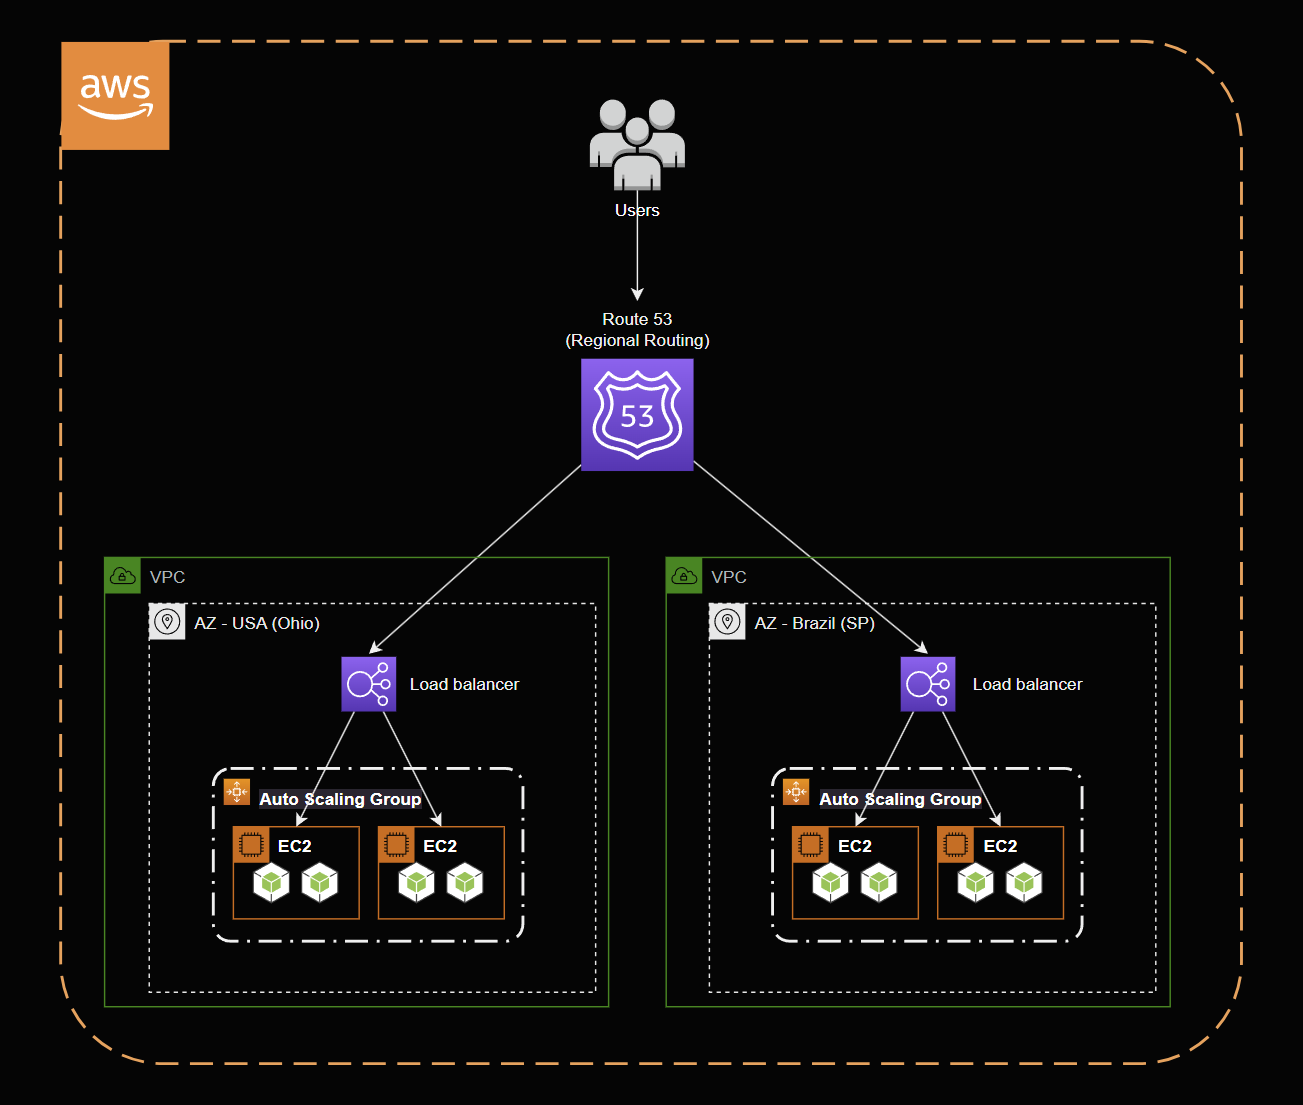
\includegraphics[width=\textwidth]{drawio/cloud-architecture.png}
    \caption{Visão Geral da Arquitetura em Nuvem}
    \label{fig:cloud-architecture}
\end{figure}

Essas práticas e tecnologias não apenas promovem a alta disponibilidade e desempenho da aplicação, mas também preparam o ambiente para escalar rapidamente em resposta às demandas crescentes, tudo sem intervenção manual, alinhando-se com as melhores práticas de DevOps e com as demandas de uma aplicação moderna.


\subsubsection{Planejamento de Infraestrutura}
% Revisado

O planejamento da infraestrutura da plataforma começou com a definição de requisitos e necessidades específicas da aplicação, que incluem:

\begin{itemize}
    \item \textbf{Baixa latência}: Para assegurar uma experiência de usuário fluida e responsiva em tempo real, a plataforma Codeboard precisa operar com baixa latência.
    \item \textbf{Alta disponibilidade}: Codeboard deve estar acessível 24/7, garantindo operação contínua, mesmo durante atualizações e manutenções.
    \item \textbf{Escalabilidade}: A plataforma deve suportar um grande número de usuários simultâneos, aumentando ou diminuindo seus recursos conforme a demanda.
    \item \textbf{Resiliência}: Codeboard precisa de mecanismos de recuperação automática frente a falhas de hardware ou software, sem impacto na experiência do usuário.
    \item \textbf{Custo-efetividade}: A infraestrutura deve ser otimizada para minimizar custos, evitando ociosidade de recursos.
    \item \textbf{Facilidade de gerenciamento}: a infraestrutura deve ser simples de gerenciar, utilizando práticas de DevOps, como \emph{Infra-as-Code} (IaC).
    \item \textbf{Segurança}: A plataforma deve ser protegida contra ameaças e ataques cibernéticos.
    \item \textbf{Monitoramento}: A plataforma deve contar com métricas e logs para acompanhar desempenho e integridade.
\end{itemize}

A hospedagem na Amazon Web Services (AWS) tornou-se uma escolha estratégica devido à sua ampla variedade de serviços, escalabilidade, confiabilidade e presença global de data centers. A infraestrutura global da AWS habilita a arquitetura \emph{Multi-Region Active-Active}, crucial para atender aos requisitos de desempenho e disponibilidade descritos.  Além disso, o \emph{free tier} da AWS foi um diferencial importante, possibilitando o desenvolvimento e os testes iniciais sem custos significativos.

Para atender a esses requisitos, foram escolhidos os seguintes serviços da AWS para compor a infraestrutura da plataforma Codeboard:

\begin{itemize}
    \item \textbf{Amazon Elastic Compute Cloud (EC2)}: Fornece instâncias virtuais escaláveis e seguras para execução da aplicação.
    \item \textbf{Amazon Elastic Load Balancing (ELB)}: Distribui o tráfego entre instâncias EC2, garantindo alta disponibilidade e escalabilidade.
    \item \textbf{AWS Auto Scaling}: Ajusta automaticamente a capacidade das instâncias EC2 conforme a demanda.
    % \item \textbf{Amazon DocumentDB}: serviço de banco de dados NoSQL que fornece instâncias gerenciadas de bancos de dados MongoDB.
    % \item \textbf{Amazon ElastiCache}: serviço de cache em memória que fornece instâncias gerenciadas de Redis.
    \item \textbf{Amazon Virtual Private Cloud (VPC)}: Cria uma rede virtual com sub-redes privadas, gateways de internet e regras de firewall.
    \item \textbf{Amazon Route 53}: Configura registros de DNS, oferece balanceamento de carga entre regiões geográficas e failover.
    \item \textbf{Amazon CloudWatch}: Proporciona métricas, logs e alarmes para monitorar a saúde e o desempenho da aplicação.
    \item \textbf{AWS Identity and Access Management (IAM)}: Gerencia o controle de acesso, permitindo a criação de usuários, grupos e políticas.
    \item \textbf{AWS Certificate Manager (ACM)}: Facilita a criação, renovação e implantação de certificados SSL/TLS para segurança de dados.
\end{itemize}

Essas escolhas de serviço atendem diretamente às necessidades de desempenho, segurança e custo, alinhando a infraestrutura às metas de alta disponibilidade e resiliência exigidas pela plataforma.


\subsubsection{Implementação de Infraestrutura como Código com Terraform}
% Revisado

Para assegurar um processo de implantação de infraestrutura que seja eficiente, escalável e replicável, a plataforma Codeboard utiliza o \emph{Terraform} como ferramenta de \emph{Infrastructure as Code} (IaC).

A utilização do Terraform como IaC garante que a infraestrutura seja declarativa e executada de forma idempotente, o que significa que recursos existentes não são recriados desnecessariamente a cada execução. Isso resulta em um gerenciamento mais eficiente dos recursos e em um controle de mudanças mais preciso. Foram estabelecidos módulos para tratar de diferentes aspectos da infraestrutura, como rede, segurança e recursos de computação, permitindo que seja possível trabalhar isoladamente em partes distintas da arquitetura sem necessidade de intervenção manual entre essas partes.


\subsection{Infraestrutura de Computação}

Dada a adoção do modelo \emph{Multi-Region Active-Active}, a infraestrutura de computação da Codeboard foi arquitetada para operar de maneira distribuída através de diferentes regiões geográficas da AWS. Essa abordagem garante, além de uma resposta eficiente a eventuais falhas regionais, uma proximidade maior com os usuários, o que ajuda a reduzir a latência. A infraestrutura de computação integra múltiplos componentes, incluindo instâncias EC2, balanceamento de carga, escalabilidade automática, monitoramento, e diversos mecanismos para segurança e recuperação de falhas, criando um ambiente robusto que sustenta a operação contínua e eficiente da plataforma Codeboard.

\subsubsection{Servidor Virtual}
% Revisado

Para hospedar a aplicação da plataforma Codeboard, foram escolhidas instâncias EC2 do tipo \emph{t3.micro}, adequadas ao estudo de caso pelos seguintes motivos: 

\begin{itemize}
    \item \textbf{Custo}: As instâncias t3.micro fazem parte do \emph{free tier} da AWS, oferecendo 12 meses de uso gratuito, o que torna essa opção financeiramente viável para a fase inicial do projeto.
    \item \textbf{Desempenho Escalável}: Com capacidade de burst, essas instâncias podem fornecer recursos adicionais de CPU temporariamente, sem custos extras, atendendo a picos de demanda.
    \item \textbf{2 vCPUs}: As instâncias t3.micro possuem 2 vCPUs, que é o mínimo recomendado para a aplicação da plataforma Codeboard, que opera em um \emph{cluster} de processos, onde cada processo é uma aplicação Node.js que é responsável pelo backend.
    \item \textbf{1 GB de memória RAM}: A memória de 1 GB é adequada para a Codeboard, pois sua função de intermediação de mensagens em tempo real requer um baixo consumo de memória.
    \item \textbf{Armazenamento em disco SSD}: Embora a Codeboard não faça uso intensivo de disco, o armazenamento SSD nas instâncias t3.micro oferece maior velocidade e confiabilidade, beneficiando a estabilidade do sistema.
\end{itemize}

As instâncias EC2 foram configuradas com o sistema operacional \emph{Ubuntu 24.04 LTS}, o servidor web \emph{NGINX}, o gerenciador de processos \emph{PM2} e outras ferramentas para auxiliar no processo de configuração da instância: \emph{Git}, \emph{Node.js}, \emph{NPM} e \emph{CertBot}. A escolha do Ubuntu 24.04 LTS deve-se à sua estabilidade e suporte de longo prazo para atualizações de segurança. O NGINX atua como um servidor web reverso, redirecionando o tráfego HTTPS para os processos Node.js que executam a Codeboard. Já o PM2 gerencia esses processos, mantendo-os ativos e reiniciando automaticamente em caso de falhas.

\subsection{Balanceamento de Carga, Escalabilidade e Recuperação de Falhas}
% Revisado

A arquitetura da plataforma Codeboard foi projetada com uma estratégia de balanceamento de carga, escalabilidade e recuperação de falhas que abrange múltiplos níveis de operação, assegurando alta disponibilidade, baixa latência e resiliência. Esta seção apresenta a abordagem utilizada para distribuir de forma eficiente o tráfego e garantir que a aplicação responda de maneira otimizada, mesmo em cenários de alta demanda ou falhas inesperadas.

Em primeiro lugar, o balanceamento de carga entre processos permite uma distribuição equitativa das requisições entre processos individuais da aplicação, garantindo o uso eficiente dos recursos da instância. Para lidar com o tráfego em servidores múltiplos, foi configurado um segundo nível de balanceamento de carga que distribui as requisições entre instâncias EC2 da AWS, de modo que a aplicação possa escalar horizontalmente conforme a demanda. Por fim, para maximizar a disponibilidade global e reduzir a latência para usuários em diferentes localidades, foi implementado um balanceamento de carga geográfico entre regiões da AWS, utilizando o Route 53 para redirecionar o tráfego para a região mais próxima do usuário.

Além disso, mecanismos de recuperação automática de falhas foram configurados em cada nível. Esses mecanismos monitoram continuamente a saúde dos processos e das instâncias, substituindo automaticamente recursos que falhem e garantindo a continuidade da aplicação. Essa estrutura multissetorial de balanceamento e recuperação permite que a plataforma Codeboard mantenha uma operação robusta e confiável, capaz de lidar com flutuações de carga e com interrupções inesperadas.

\subsubsection{Balanceamento de Carga entre Processos}
% Revisado

A aplicação Codeboard opera em um \emph{cluster} de processos, o que torna o balanceamento de carga essencial para distribuir o tráfego de entrada de maneira eficiente. Para isso, o PM2 foi configurado no modo cluster, permitindo a criação de múltiplos processos Node.js que compartilham o mesmo \emph{socket} de rede. Dessa forma, o NGINX redireciona o tráfego entre os processos por meio do módulo \emph{proxy\_pass}, que envia as requisições HTTP para o processo Node.js que executa a Codeboard.

O algoritimo de balanceamento de carga utilizado é o \emph{Round Robin}, que distribui o tráfego de entrada de forma alternada entre os processos do cluster, assegurando que cada processo receba uma quantidade igual de solicitações. A Figura \ref{fig:round-robin-load-balancing} ilustra o funcionamento do algoritmo Round Robin, enquanto a Figura \ref{fig:pm2-cluster-mode} mostra o modo cluster do PM2 em ação.

\begin{figure}[H]
    \centering
    \includegraphics[width=\textwidth]{diagrams/round-robin-load-balancing.png}
    \caption{Balanceamento de Carga com Round Robin}
    \label{fig:round-robin-load-balancing}
\end{figure} 

\begin{figure}[H]
    \centering
    \includegraphics[width=\textwidth]{diagrams/pm2-cluster-mode.png}
    \caption{Modo Cluster do PM2}
    \label{fig:pm2-cluster-mode}
\end{figure}

O balanceamento de carga entre processos otimiza o uso dos recursos de CPU e memória, distribuindo a carga de trabalho de maneira uniforme entre os vCPUs das instâncias EC2, garantindo um desempenho estável e eficiente.

\subsubsection{Recuperação Automática de Falhas em Processos}
% Revisado

O balanceamento de carga entre processos também contribui para a alta disponibilidade e confiabilidade da aplicação. Em caso de falha de um dos processos, o tráfego é automaticamente redirecionado para outros, evitando interrupções para os usuários.

Para reforçar a tolerância a falhas e garantir a alta disponibilidade, foram configurados no PM2 mecanismos de monitoramento e recuperação automática. Esse monitoramento verifica continuamente os processos Node.js e, ao detectar uma falha, reinicia o processo comprometido. A Figura\ref{fig:pm2-fault-tolerance} ilustra o funcionamento do monitoramento e recuperação de falhas pelo PM2, garantindo que a aplicação permaneça em funcionamento mesmo diante de falhas pontuais.


\begin{figure}[H]
    \centering
    \includegraphics[width=0.75\textwidth]{diagrams/pm2-fault-tolerance.png}
    \caption{Tolerância à Falhas com PM2}
    \label{fig:pm2-fault-tolerance}
\end{figure}


\subsubsection{Balanceamento de Carga entre os Servidores}
% Revisado

A infraestrutura de computação da plataforma Codeboard foi projetada para ser distribuída e redundante, assegurando que o tráfego seja balanceado entre várias instâncias EC2 e entre diferentes regiões geográficas. Para essa finalidade, utilizou-se o AWS Elastic Load Balancing (ELB), que distribui o tráfego de entrada de forma equilibrada entre as instâncias, garantindo alta disponibilidade e escalabilidade da aplicação.

Entre os tipos de ELB disponíveis, como o Application Load Balancer (ALB), Network Load Balancer (NLB) e Classic Load Balancer (CLB), escolheu-se o ALB. Esse balanceador de camada 7 permite o roteamento de tráfego com base em critérios específicos, como URL, cabeçalhos HTTP e métodos HTTP. O ALB foi configurado com um certificado SSL para assegurar a segurança do tráfego HTTPS entre clientes e servidores.

O algoritmo de balanceamento de carga adotado foi o \emph{Round Robin}, que distribui o tráfego de forma equitativa entre as instâncias EC2, garantindo uma divisão equilibrada de requisições.


% TODO: Voltar no capítulo 3 para explicar a importância do Health Check? Testar se a conexão com o banco de dados está funcionando, se a aplicação está respondendo, etc.

Para garantir que apenas instâncias saudáveis recebam tráfego, foram configurados \emph{Health Checks} para monitorar a saúde das instâncias EC2. Os Health Checks realizam verificações periódicas em uma rota específica da aplicação Codeboard, permitindo que o ELB detecte se cada instância está respondendo corretamente. Se uma instância não responder adequadamente ao Health Check, o ELB a marca como indisponível e redireciona o tráfego para outras instâncias saudáveis.

Configurou-se o Health Check com um intervalo de 30 segundos e um tempo limite de 5 segundos, o que significa que o ELB realiza uma verificação a cada 30 segundos e aguarda uma resposta dentro de 5 segundos. Após duas falhas consecutivas, a instância é marcada como indisponível e o tráfego é redirecionado para outras instâncias saudáveis. A Figura \ref{fig:elb-health-check} ilustra o funcionamento do Health Check do ELB.

\begin{figure}[H]
    \centering
    \includegraphics[width=0.75\textwidth]{diagrams/elb-health-check.png}
    \caption{Health Check do ELB}
    \label{fig:elb-health-check}
\end{figure}


\subsubsection{Escalabilidade Horizontal com Auto Scaling}
% Revisado

Para garantir a alta disponibilidade da plataforma Codeboard, a infraestrutura foi projetada para escalar horizontalmente, permitindo que a aplicação aumente ou reduza seus recursos de acordo com a demanda, sem necessidade de intervenção manual. Essa escalabilidade automática foi implementada com o AWS Auto Scaling, que ajusta a quantidade de instâncias EC2 com base na utilização de recursos.

O Auto Scaling utiliza um Auto Scaling Group (ASG) para monitorar a utilização de CPU nas instâncias EC2 e ajustar a quantidade de instâncias conforme uma política de escalabilidade. Definiram-se gatilhos específicos: quando a utilização de CPU ultrapassa um limite predefinido, uma nova instância é adicionada ao grupo, distribuindo melhor a carga. Inversamente, se a utilização de CPU cair abaixo de um limite, o ASG reduz o número de instâncias, otimizando custos. Foi configurado um número mínimo e máximo de instâncias, garantindo um custo controlado e uma capacidade mínima sempre disponível. A Figura \ref{fig:auto-scaling-horizontal-scalability} ilustra essa escalabilidade horizontal com o Auto Scaling.

\begin{figure}[H]
    \centering
    \includegraphics[width=\textwidth]{diagrams/auto-scaling-horizontal-scalability.png}
    \caption{Escalabilidade Horizontal com Auto Scaling Group}
    \label{fig:auto-scaling-horizontal-scalability}
\end{figure}

Os limites de gatilhos de escalabilidade foram definidos com base em testes e monitoramento da aplicação, estabelecendo 70\% de uso de CPU para adicionar uma nova instância e 30\% para removê-la. Os valores de instâncias mínima e máxima foram configurados entre 1 e 5, podendo ser ajustáveis conforme previsões de tráfego, sazonalidade e eventos especiais.

\subsubsection{Recuperação Automática de Falhas em Servidores}
% Revisado

O Auto Scaling do AWS também possui um mecanismo de recuperação automática de falhas, que monitora continuamente a saúde das instâncias EC2. Quando uma instância é marcada como indisponível pelo ELB (por falhar em um Health Check), o Auto Scaling substitui automaticamente a instância defeituosa por uma nova, garantindo que a aplicação da plataforma Codeboard permaneça sempre disponível e resiliente a falhas. Essa combinação de Auto Scaling, ELB e PM2 resulta em uma arquitetura altamente disponível, escalável e confiável. A Figura \ref{fig:auto-scaling-fault-tolerance} ilustra o funcionamento da recuperação automática de falhas com o Auto Scaling.

\begin{figure}[H]
    \centering
    \includegraphics[width=\textwidth]{diagrams/auto-scaling-fault-tolerance.png}
    \caption{Recuperação Automática de Falhas com Auto Scaling}
    \label{fig:auto-scaling-fault-tolerance}
\end{figure}

Durante a inicialização de uma nova instância, o Auto Scaling aplica um \emph{warmup time} de 180 segundos, período necessário para que a instância esteja completamente operacional. Nesse tempo, são realizadas tarefas como configuração da instância, inicialização da aplicação e estabelecimento de conexões com o banco de dados. Durante o warmup time, a instância permanece indisponível para o ELB, e o tráfego é direcionado para outras instâncias saudáveis. Após o término do warmup, a instância é marcada como disponível e começa a receber tráfego. Esse warmup time ajuda a evitar interrupções na aplicação, garantindo que apenas instâncias totalmente preparadas participem da distribuição de carga.


\subsubsection{Balanceamento de Carga entre Regiões Geográficas}
% Revisado

A infraestrutura da plataforma Codeboard foi projetada para operar em várias regiões geográficas da AWS, permitindo distribuição do tráfego de usuários entre essas regiões para assegurar alta disponibilidade e baixa latência. Essa configuração de várias regiões não só oferece resiliência em caso de falhas regionais (devido a desastres naturais, falhas de hardware, ou manutenção programada), mas também aproxima a aplicação dos usuários, o que reduz a latência e aprimora a experiência de uso.

Para essa distribuição de tráfego entre regiões, foi configurado o Amazon Route 53, o serviço de DNS da AWS que também oferece balanceamento de carga e failover. Um registro de DNS foi criado para a aplicação da plataforma Codeboard no Route 53, o qual direciona o tráfego para o ELB de cada região geográfica. Devido à natureza de comunicação em tempo real da plataforma, o Route 53 foi configurado com balanceamento de carga baseado em latência, de forma que redireciona o tráfego para a região geográfica mais próxima do usuário, garantindo uma experiência rápida e eficiente. 

\begin{figure}[H]
    \centering
    \includegraphics[width=\textwidth]{diagrams/route-53-geographic-load-balancing.png}
    \caption{Balanceamento de Carga Baseado em Latência com Route 53}
    \label{fig:route-53-geographic-load-balancing}
\end{figure}

A Figura \ref{fig:route-53-geographic-load-balancing} demonstra o funcionamento do balanceamento de carga baseado em latência do Route 53. Quando um usuário faz uma solicitação DNS, o Route 53 primeiro identifica a localização geográfica do usuário com base em seu endereço IP. Em seguida, redireciona o tráfego para a região mais próxima, que consequentemente possui a menor latência, melhorando a experiência do usuário. Esse balanceamento de carga geográfico garante que a plataforma opere de forma eficiente, independentemente da localização dos usuários.

\subsection{Segurança da Infraestrutura}
% Revisado

A segurança da infraestrutura é um aspecto essencial para garantir a proteção dos dados e a continuidade das operações da plataforma Codeboard. Nesta seção, são discutidas as medidas de segurança implementadas para prevenir acesso não autorizado, proteger o tráfego de dados e garantir a confiabilidade da infraestrutura. Essas práticas abrangem desde o controle de acesso aos recursos de computação até a aplicação de criptografia de dados, assegurando a integridade e a privacidade das informações dos usuários. 

\subsubsection{Controle de Acesso}
% Revisado

Para proteger a infraestrutura computacional da plataforma Codeboard, várias políticas de segurança foram implementadas, incluindo:

\begin{itemize}
    \item \textbf{AWS Identity and Access Management (IAM)}: políticas e papéis no IAM foram criados para controlar o acesso aos recursos da AWS, aplicando o princípio do menor privilégio. As instâncias EC2, por exemplo, possuem permissões restritas, limitadas apenas às ações necessárias para o funcionamento da aplicação.
    \item \textbf{Firewall}: regras de firewall foram configuradas no \emph{Security Group} da VPC para restringir o tráfego de entrada e saída das instâncias EC2. Somente as portas essenciais para a aplicação estão abertas: a porta 80 (HTTP) é acessível apenas pelo ELB, enquanto a porta 22 (SSH) está disponível exclusivamente para IPs autorizados. Todas as demais portas de entrada são bloqueadas.
    \item \textbf{Chaves SSH}: chaves SSH foram geradas para garantir a autenticação segura de usuários no acesso remoto às instâncias EC2.
\end{itemize}

Além disso, as instâncias EC2 não são acessadas diretamente; o tráfego de entrada passa pelo ELB, que distribui as conexões de forma uniforme. O ELB está configurado com um certificado SSL para garantir a criptografia do tráfego entre cliente e servidor, protegendo os dados em trânsito. Seu Security Group permite apenas o tráfego de entrada na porta 443 (HTTPS).

\subsubsection{Criptografia de Dados em Trânsito}
% Revisado

Para assegurar a segurança dos dados em trânsito, um certificado SSL foi configurado no ELB para criptografar o tráfego entre o cliente e o servidor. Esse certificado, emitido pelo AWS Certificate Manager (ACM), é gratuito e gerenciado, sendo adequado para serviços da AWS. A configuração inclui um domínio personalizado da plataforma Codeboard, disponível em https://codeboard.pitrol.dev/, o que garante a autenticidade e a integridade das conexões HTTPS. Com isso, a criptografia dos dados em trânsito protege contra interceptações e garante a privacidade e a segurança dos usuários.

% TODO?: \subsubsection{Rotatividade de Chaves e Segredos}

\subsection{Banco de Dados MongoDB}
% Revisado

O banco de dados escolhido para a plataforma Codeboard foi o MongoDB, uma solução NoSQL amplamente utilizada por sua flexibilidade, escalabilidade e alto desempenho em aplicações modernas. Diversas abordagens poderiam ser adotadas para hospedar o MongoDB, incluindo instalações locais, máquinas virtuais, contêineres Docker e serviços gerenciados na nuvem. No caso da Codeboard, optou-se pelo \emph{MongoDB Atlas}, um serviço gerenciado pela própria MongoDB que opera sobre infraestruturas robustas como a AWS, Google Cloud Platform e Microsoft Azure.

Essa escolha trouxe diversas vantagens, incluindo alta disponibilidade, escalabilidade e segurança integradas. O MongoDB Atlas proporciona funcionalidades como backups automáticos, monitoramento em tempo real, escalabilidade ajustável e criptografia de dados em trânsito e em repouso, além de integração com outros serviços da AWS. Para atender às necessidades iniciais da aplicação, foi selecionada a instância \emph{M10}, que oferece 2 GB de armazenamento e 0,5 GB de RAM, com suporte a escalabilidade para acomodar futuras demandas.

A adoção do MongoDB Atlas permite que a equipe foque no desenvolvimento da aplicação, enquanto a gestão do banco de dados é simplificada por meio de recursos automatizados, garantindo a robustez e a eficiência no gerenciamento dos dados da plataforma.


\subsubsection{Escalabilidade Vertical Automática}
% Revisado

O banco de dados MongoDB da plataforma Codeboard foi configurado para escalar verticalmente de maneira automática, garantindo que possa atender ao crescimento das demandas de forma eficiente. A escalabilidade vertical consiste em aumentar os recursos de uma única instância, como CPU, memória e armazenamento, sem a necessidade de configurar múltiplas réplicas ou lidar com a complexidade da escalabilidade horizontal.

A escolha pela escalabilidade vertical, em vez da horizontal, foi fundamentada por duas razões principais:
\begin{enumerate}
    \item \textbf{Custo e Complexidade}: A escalabilidade horizontal envolve a distribuição de dados e cargas de trabalho entre múltiplas instâncias, o que requer configurações avançadas e ferramentas específicas, como sharding. Para um banco de dados com baixa utilização de recursos, a escalabilidade horizontal representaria um custo desnecessário e maior complexidade operacional.
    \item \textbf{Adequação ao Escopo Atual}: O uso inicial da instância M10 do MongoDB Atlas, com 2 GB de armazenamento e 0,5 GB de RAM, provou ser suficiente para as necessidades da aplicação. No entanto, a escalabilidade vertical automática garante que, conforme a demanda cresça, a infraestrutura acompanhe esse crescimento sem interrupções.
\end{enumerate}

O MongoDB Atlas permite configurar a escalabilidade vertical de forma automática, ajustando a capacidade da instância com base na utilização de recursos. Os gatilhos predefinidos monitoram métricas de desempenho, como:
\begin{itemize}
    \item \textbf{CPU}: Se a utilização ultrapassar um limite definido de 75\% na última hora, a capacidade da instância é aumentada automaticamente.
    \item \textbf{Memória}: Um uso persistente acima de uma faixa segura de 90\% por pelo menos 10 minutos dispara o aumento de recursos.
    \item \textbf{Armazenamento}: Quando o espaço disponível atinge um limite crítico de 90\%, a capacidade de armazenamento é ampliada. 
\end{itemize}


Da mesma forma, a escalabilidade vertical também reduz a capacidade da instância quando os recursos são subutilizados, ajudando a otimizar custos operacionais sem sacrificar o desempenho. A Figura \ref{fig:mongodb-atlas-vertical-scalability} ilustra o funcionamento da escalabilidade vertical automática configurada no MongoDB Atlas.

\begin{figure}[H]
    \centering
    \includegraphics[width=\textwidth]{diagrams/mongodb-atlas-vertical-scalability.png}
    \caption{Escalabilidade Vertical Automática no MongoDB Atlas}
    \label{fig:mongodb-atlas-vertical-scalability}
\end{figure} 

Os benefícios da escalabilidade vertical automática no MongoDB Atlas são diversos e contribuem significativamente para a eficiência operacional da plataforma Codeboard, diminuindo a complexidade, reduzindo custos e automatizando o gerenciamento de recursos do banco de dados. Essa abordagem garante que o banco esteja sempre preparado para atender às demandas crescentes da aplicação, sem a necessidade de interrupções ou intervenções manuais.


\subsubsection{Backup, Controle de Acesso e Segurança de Dados}
% Revisado

Para atender aos requisitos de segurança e confiabilidade da plataforma Codeboard, foi implementada uma estratégia robusta que abrange tanto o gerenciamento de backups quanto o controle de acesso ao banco de dados e a proteção dos dados em trânsito e em repouso.

Os backups automáticos realizados pelo MongoDB Atlas garantem a preservação e recuperação de dados em caso de falhas ou perdas acidentais, com uma política de retenção que permite a restauração para pontos no tempo ao longo de 14 dias. Adicionalmente, backups sob demanda oferecem flexibilidade para proteger os dados em momentos críticos, como antes de atualizações ou mudanças significativas.

No que diz respeito à segurança, políticas rigorosas de controle de acesso foram implementadas para restringir conexões não autorizadas. Isso inclui o uso de \emph{Whitelists} de IPs e autenticação com credenciais específicas para diferentes níveis de permissão. Além disso, a criptografia de dados, tanto em trânsito quanto em repouso, protege contra interceptações e acessos indevidos, utilizando tecnologias SSL e armazenamento seguro no MongoDB Atlas.

Essas medidas asseguram que os dados da plataforma permaneçam seguros, disponíveis e protegidos contra uma ampla gama de riscos e ameaças.

\subsection{Banco de dados Redis}
% Revisado

O Redis desempenha um papel crucial na infraestrutura da plataforma Codeboard, servindo como um banco de dados chave-valor em memória de alta performance. Sua velocidade, simplicidade e capacidade de escalabilidade o tornam ideal para atender às necessidades de aplicações que exigem processamento rápido de dados em tempo real, como é o caso da Codeboard. Nesta seção, serão explorados os detalhes de sua configuração, os benefícios de utilizar uma solução gerenciada e as práticas implementadas para garantir a segurança, disponibilidade e desempenho do banco de dados.

\subsubsection{Provedor de Banco de Dados}
% Revisado

O banco de dados Redis da plataforma Codeboard está hospedado no \emph{Redis Cloud}, uma solução gerenciada pela própria Redis. Essa escolha foi motivada pela robustez e confiabilidade do serviço, que elimina a necessidade de gerenciamento manual da infraestrutura de banco de dados, além de oferecer recursos avançados como monitoramento, backup e suporte técnico especializado.

O Redis Cloud proporciona uma infraestrutura otimizada para alta disponibilidade e desempenho, com suporte a escalabilidade automática para lidar com variações de carga. Além disso, o uso de uma solução gerenciada permite que a equipe foque no desenvolvimento e na operação da aplicação, ao invés de dedicar tempo e recursos ao gerenciamento do banco de dados.

\subsubsection{Sharding e Replicação}
% Revisado

Para garantir alta disponibilidade e baixa latência, o Redis foi configurado com sharding e replicação. A abordagem de escalabilidade horizontal, baseada no sharding, distribui os dados entre múltiplas réplicas em diferentes nós, permitindo que o banco de dados suporte um grande volume de transações simultâneas sem comprometer o desempenho.

O sharding foi configurado de forma automática pelo Redis Cloud, que gerencia a alocação de dados e o balanceamento de carga entre shards. Já a replicação assegura a resiliência do sistema, criando réplicas secundárias de cada shard. Em caso de falha de um nó, o Redis Cloud promove automaticamente uma réplica para substituí-lo, garantindo continuidade no serviço.

\subsubsection{Controle de Acesso e Segurança}
% Revisado

A segurança do banco de dados Redis foi configurada com foco em prevenir acessos não autorizados e proteger os dados transmitidos. As políticas de controle de acesso incluem autenticação por senha e restrições baseadas em IP, permitindo conexões apenas de hosts autorizados. Essa abordagem reduz significativamente o risco de acessos externos indevidos.

Para garantir a proteção dos dados em trânsito, o tráfego entre os clientes e o Redis é criptografado utilizando TLS, prevenindo interceptações e acessos maliciosos.

Dado o papel do Redis na plataforma Codeboard, que é utilizado principalmente para dados temporários, não foram configurados backups automáticos. Os dados críticos da aplicação são armazenados no MongoDB, que conta com backups automáticos e políticas de retenção robustas. Essa estratégia assegura que, mesmo em caso de perda de dados no Redis, eles possam ser facilmente regenerados sem impacto significativo na operação.


\subsection{Distribuição de Conteúdo (CDN)}
% Revisado

Uma \emph{Content Delivery Network} (CDN) é uma rede de servidores distribuídos geograficamente que trabalham em conjunto para entregar conteúdos da web com rapidez e eficiência. Ao armazenar cópias dos arquivos em locais próximos aos usuários finais, uma CDN reduz o tempo de carregamento, diminui a carga no servidor de origem e melhora a experiência do usuário.

\subsubsection{Plataforma de CDN}
% Revisado

A utilização de uma CDN desempenha um papel essencial na entrega rápida e eficiente do front-end da plataforma Codeboard. A infraestrutura foi implementada utilizando a plataforma \emph{Vercel}, que combina os benefícios de uma CDN global com recursos de plataforma como serviço (PaaS), otimizando a experiência dos usuários finais.

O uso da CDN integrada ao Vercel traz diversos benefícios, incluindo:

\begin{itemize}
    \item Redução de latência: Ao distribuir o conteúdo para servidores localizados próximos aos usuários, o tempo de resposta é minimizado.
    \item Alta disponibilidade: A CDN utiliza redundância para garantir que os conteúdos estejam sempre acessíveis, mesmo em caso de falhas em servidores específicos.
    \item Escalabilidade automática: A infraestrutura da CDN lida automaticamente com picos de tráfego, assegurando desempenho consistente.
    \item Segurança aprimorada: Recursos como mitigação de DDoS e controle de acesso a nível de borda ajudam a proteger a plataforma contra ataques.
\end{itemize}

\subsubsection{Configuração da CDN}
% Revisado

No contexto da Codeboard, a configuração da CDN foi simplificada pela utilização do Vercel. A plataforma automaticamente gerencia o cache de conteúdo estático e implementa o cache dinâmico conforme necessário, baseado nos cabeçalhos de resposta configurados na aplicação. Regras de invalidade de cache são aplicadas automaticamente durante os deploys, garantindo que os usuários sempre acessem a versão mais recente da aplicação.

Além disso, a CDN do Vercel está totalmente integrada com o sistema de build e deploy contínuos, sincronizando alterações no front-end com a rede de distribuição em tempo real. Essa abordagem garante alta performance e agilidade no lançamento de novas funcionalidades.


\subsection{Monitoramento}
% Revisado

% Por que monitoramento é importante? R: Garantir a disponibilidade, desempenho e segurança da aplicação, atuando proativamente para evitar falhas e interrupções.

O monitoramento é um elemento crítico para garantir a disponibilidade, o desempenho e a segurança da aplicação. Por meio do acompanhamento contínuo de métricas e logs, é possível identificar e mitigar problemas proativamente, antes que causem interrupções ou degradação no serviço. Esta seção detalha como o monitoramento é implementado na plataforma Codeboard, abrangendo tanto a aplicação quanto os recursos de infraestrutura em nuvem.

\subsubsection{Monitoramento da Aplicação}
% Revisado

% Como o monitoramento da aplicação é feito? R: CloudWatch
% Quais métricas são monitoradas? R: Requisições, logs de erros, etc.

O monitoramento da aplicação é realizado utilizando o \emph{Amazon CloudWatch}, um serviço nativo da AWS que permite coletar, analisar e agir com base em dados e logs de desempenho. As métricas monitoradas incluem:

\begin{itemize}
    \item \textbf{Requisições}: Número de requisições recebidas, permitindo analisar padrões de tráfego e identificar possíveis gargalos.
    \item \textbf{Logs de erros}: Registro de falhas e exceções capturados em tempo real, possibilitando a identificação de problemas no código ou na infraestrutura.
    \item \textbf{Latência}: Tempo médio de resposta das requisições, monitorando a eficiência da aplicação e identificando possíveis pontos de melhoria.
\end{itemize}

Os dados coletados são apresentados em dashboards personalizados, oferecendo uma visão consolidada da saúde da aplicação e facilitando a identificação de padrões anormais.


\subsubsection{Monitoramento de Recursos da Nuvem}
% Revisado

% Como o monitoramento de recursos da nuvem é feito? R: CloudWatch
% Quais métricas são monitoradas? R: CPU, memória, etc.

Além da aplicação, os recursos da infraestrutura de computação em nuvem também são monitorados por meio do Amazon CloudWatch. Essa abordagem assegura que os componentes subjacentes, como os servidores, operem dentro dos parâmetros esperados.

As principais métricas monitoradas incluem:

\begin{itemize}
    \item \textbf{Uso de CPU}: Percentual de utilização do processador, indicando se os recursos estão sendo subutilizados ou sobrecarregados.
    \item \textbf{Uso de memória}: Quantidade de memória consumida, essencial para evitar problemas de desempenho devido à falta de recursos.
    \item \textbf{Tamanho de disco}: Utilização de armazenamento, permitindo antecipar a necessidade de expansão.
\end{itemize}

O monitoramento desses recursos é fundamental para identificar gargalos de desempenho e escalonar a infraestrutura de maneira eficiente.

\subsubsection{Alertas e Notificações}
% Revisado

O sistema de monitoramento da plataforma Codeboard conta com uma estratégia robusta de alertas para garantir respostas rápidas a possíveis incidentes. Os alertas são configurados no Amazon CloudWatch, permitindo a detecção e notificação de anomalias em tempo real.

As principais características do sistema de alertas incluem critérios personalizáveis, permitindo a configuração de limites para métricas específicas, como latência acima de 500ms, uso de CPU superior a 80\% ou erros 5xx que excedam um determinado volume. Além disso, há integração com ferramentas de comunicação, com notificações automáticas enviadas para canais como Slack e e-mail, garantindo que os responsáveis sejam informados imediatamente.

Com essa abordagem, o sistema de alertas fortalece a capacidade da plataforma de reagir rapidamente a eventos adversos, reduzindo o impacto nos usuários e assegurando a continuidade do serviço.

\section{Testes e Resultados}

TODO: Importância dos testes voltados à infraestrutura.

TODO: Objetivo do capítulo: validar a escalabilidade, tolerância a falhas, desempenho e segurança da plataforma Codeboard UERJ.

\subsection{Testes de Escalabilidade}

\subsubsection{Escalabilidade Horizontal}

\subsubsection{Escalabilidade Vertical}

\subsection{Testes de Tolerância a Falhas}

\subsubsection{Falhas em Servidores}

\subsubsection{Recuperação Automática}

\subsubsection{Falha em Regiões Geográficas}

\subsection{Testes de Desempenho}

\subsubsection{Tempo de Resposta}

\subsubsection{Desempenho do Redis}

\subsubsection{Desempenho do MongoDB}

\subsection{Testes de Segurança}

\subsubsection{Testes de Firewall}

\subsubsection{Ataques de DDoS}

\subsubsection{Criptografia}

\subsection{Testes de Monitoramento}

\subsubsection{Monitoramento de Recursos}

\subsubsection{Alertas de Incidentes}




\backmatter

%=====================================================================
% Referencias via BibTeX
%=====================================================================
\citeoption{abnt-options4}
\bibliography{bibliography/references}


%=====================================================================
\end{document}